\documentclass{mcmthesis}
\mcmsetup{CTeX = false,   % 使用 CTeX 套装时,设置为 true
        tcn = 2221805, problem = C,
        sheet = true, titleinsheet = true, keywordsinsheet = true,
        titlepage = false, abstract = true}
% sheet是摘要页(封面),titlepage是标题页(相当于去掉摘要页页眉之后剩下的),
% 需不需要得看官方说明    
\usepackage{newtxtext}%\usepackage{palatino}
\usepackage{lipsum}
\usepackage{float}
\usepackage{subfigure}	%多张图片
\usepackage{mathdots}
\usepackage{indentfirst}%首段缩进
\usepackage{indentfirst}
\usepackage{amsthm,amsmath,amssymb}
\usepackage{mathrsfs}
\usepackage{enumitem}
\usepackage{algorithm}
\usepackage{algorithmic}
\usepackage{comment}
\usepackage{algorithm}
\usepackage{algorithmic}
\usepackage{graphicx}
\usepackage{subfigure}
\usepackage{geometry}

\graphicspath{{figures/}}


\title{\textbf{Quantitative Trading: Stirring up the Storm}}
\author{team 2221805}
\date{\today}
\begin{document}
\begin{abstract}
	
Volatility and unpredictability have long been two of the most enthralling aspects of financial markets. A rational trading approach can assist traders in generating consistent profits with a low risk. In this competition, we have been asked to develop just this form of trading strategy. The specific tasks include three questions.

As for question 1, we divide the assignment into two submodules: future price predicting and investment decision. The price forecasting section begins by pre-processing the historical price stream. It consists of the following four steps: \textbf{removing nulls}, \textbf{first-order differencing}, \textbf{reconstructing dimensions}, and \textbf{normalization}. Then, we anticipate future prices using  LSTM, SVM, RandomForest, XGBoost, LightGBM, and LinearRegression, and evaluate their error levels using MSE, etc. Based on a thorough evaluation, we determine that the \textbf{LSTM} performs better and hence choose it as a predictor for further decisions. 

On the investment decision part, our core notion is to simplify the investment decision as a \textbf{optimization issue}. First, we must evaluate the best time to enter the market. \textbf{E-ratio} is a sensitive indication we use to gauge market entry. When it exceeds our criteria, the current time is regarded as eligible for investment. Then we create an \textbf{investing factor} by comparing the current and prospective portfolio returns and Sharpe ratios. It is positively correlated with the rate of return and negatively correlated with risk. That is, to construct a portfolio for tomorrow that maximizes the investment component while guaranteeing total asset growth. We use Particle Swarm Optimization (PSO) to generate the daily optimal portfolio. After a 5-year investment period, we can achieve a 129.6\% average yearly return and a total income of \$108387.309.

To answer question 2, we evaluate our strategy's performance using three metrics: \textbf{annualized rate of return}, \textbf{Sharpe Ratio}, and \textbf{maximum retracement}. Our investing method outperforms many established quantitative trading models in terms of these metrics, making it a viable optimal option.

For question 3, we undertake a \textbf{sensitivity analysis} by altering the gold and bitcoin commission ratios and observing the trend in total assets and the respective percentages of cash, gold, and bitcoin in daily portfolio holdings. We find that the percentage of holdings increases when the asset's commission decreases, and vice versa. This follows basic market principles. In addition, adjusting the gold and bitcoin commission ratios has no significant effect on the overall asset trend or value, indicating that our model is not sensitive to commission changes.

Lastly, we summarize our models, strategies and results and present them in a memo to traders with the aim that this quantitative trading system will deliver stable and sustainable returns.
\begin{keywords}
Quantitative Trading; LSTM; Trend-following strategy
\end{keywords}
\end{abstract}
\maketitle
%% Generate the Table of Contents, if it's needed.
\setcounter{page}{1}
\tableofcontents
\newpage

%%
%% Generate the Memorandum, if it's needed.
%% \memoto{\LaTeX{}studio}
%% \memofrom{Liam Huang}
%% \memosubject{Happy \TeX{}ing!}
%% \memodate{\today}
%% \logo{\LARGE I'm pretending to be a LOGO!}
%% \begin{memo}[Memorandum]
%%   \lipsum[1-3]
%% \end{memo}
%%
\section{Introduction}
\subsection{Background}

	The financial business exists to maximize revenues by distributing resources efficiently. Market traders routinely acquire and sell volatile assets to secure investments with the potential for profit maximization. Typically, traders made decisions about each transaction based on their opinions of the market. However, complexity and dynamics are increasing drastically in today's financial markets, where traditional assets (like gold) coexist with digital ones (like Bitcoin). The traditional trading strategy is often inefficient and prone to big losses due to irrational conduct\cite{learning1}.
	
	Unlike traditional approaches, quantitative trading is an automated method of profit-mining from historical market data that follows a predetermined trading strategy or logic. It outperforms human traders in terms of stability, speed, and reliability\cite{learning2}. Thus, quantitative trading algorithms can aid investors in achieving desired returns across a variety of portfolios.

\subsection{Problem Restatement}

	At the request of the trader mentioned in the problem, We need to develop a model that uses only the past stream of daily prices to date to determine daily transactions. Specifically, the investment is confined to a gold and bitcoin portfolio with a \$1000 beginning capital for a five-year commitment. Each time a transaction is made, a commission must be paid. Our goal is to reap the greatest possible profit at the cut-off day.
	
	In order to accomplish the requirement, our specific works are as follows:
	\begin{itemize}		%无序列表
		\item Based on the previous price data, predict the price of gold or bitcoin for the day.
		\item Create a trading strategy that maximizes the 5-year benefit based on the anticipated prices determined in the previous step and the assets currently own.
		\item Confirm the quality and superiority of our model by comparing our results to those of other methods.
		\item Perform model sensitivity analysis by varying the commission amount, and investigate the influence on trading strategies and final returns of this adjustment.
		\item Write a memo to the trader summarizing our approach, model, and outcomes.
	\end{itemize}		

\subsection{Our Work}

The overview of our work is presented in Fig.\ref{fig:ourwork} , including price forecast,trading strategy,result analysis.

\begin{figure}[H]	%浮动体参数
	\centering
	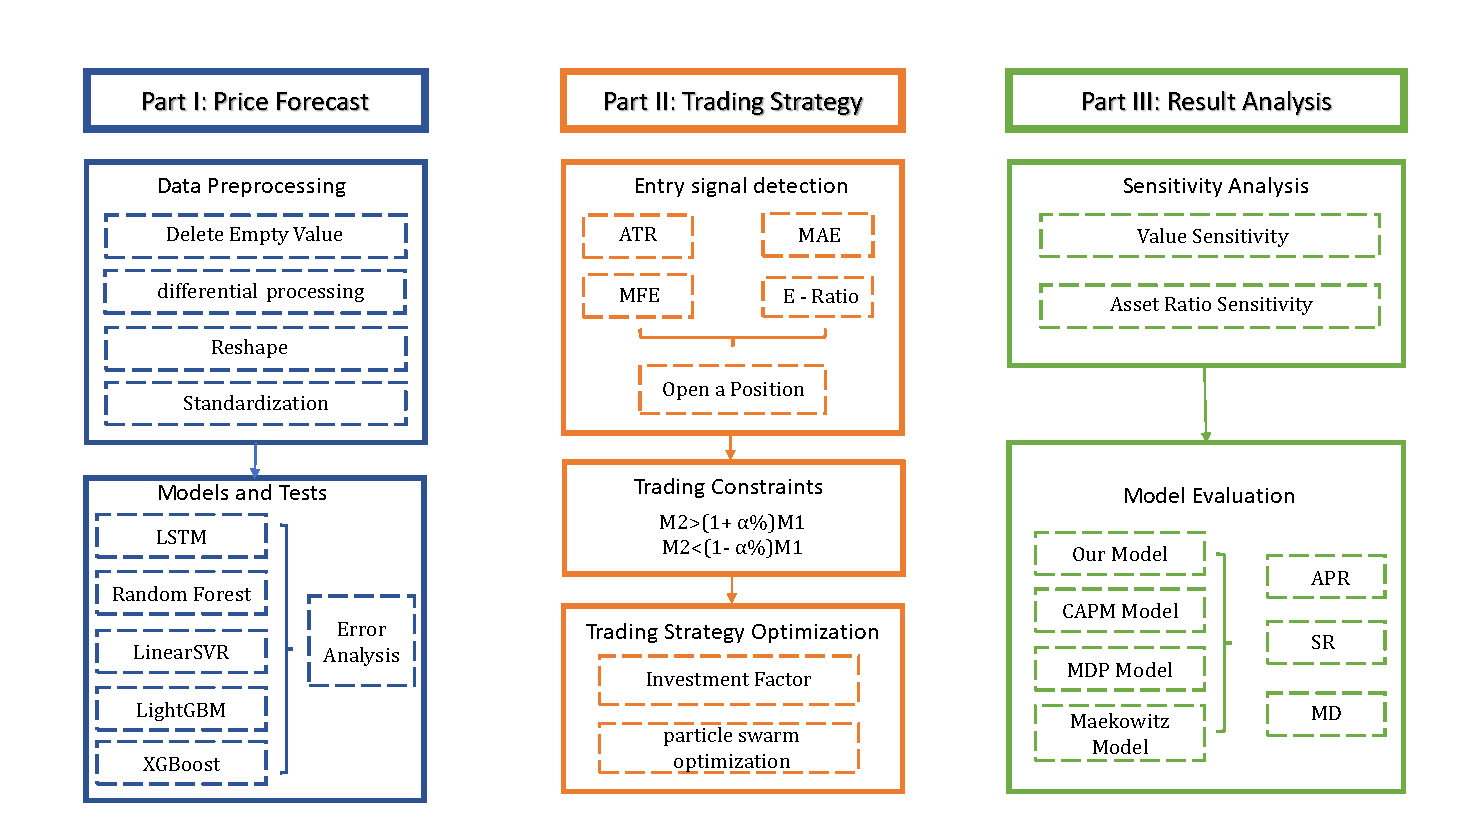
\includegraphics[width=0.9\textwidth]{ourwork}	%指定相同图片宽度,等比缩放
	\caption{Overview of ourworks} 
	\label{fig:ourwork}		%题注、引用
\end{figure}

\section{Assumptions and Justifications} 
To simplify the problem, we make the following assumptions:
\begin{enumerate}
	\item \textbf{Assume that the gold and bitcoin price series are fully determined by a time-series connection, disregarding influences such as public opinion and government policy.}
	Whereas the real price series exhibits a time series relationship, it is not entirely dependent on it and is modified by a variety of factors. However, as stated in the question, we can only forecast future pricing using historical data. That is, in this case, a forecasting model that ignores other variables is acceptable.
	
	\item \textbf{Prudent investor assumption: when making a deal, avoid spending all available cash or selling an asset (e.g. gold, bitcoin) completely short. }In this case, because both buying and selling entail fees, frequent trading of big quantities will extract a significant amount of fees, masking a decline in investment returns. A limit-based trading strategy enables investors to mitigate the negative impact of fees on the growth of the total assets.
	
	\item \textbf{The optimal strategy indicates the best strategy after evaluating the return and risk, not the strategy that takes the extreme value in one aspect.} In order to make profit in a sustainable way, the strategy must have a particular amount of risk resistance while maintaining a certain rate of return
\end{enumerate}
	

\section{Model 1: Price Forecast}
\subsection{Long and Short-Term Memory Model}
Accurate price forecasting is the first step to developing a successful trading strategy. With the help of price forecasting, we can see where prices are headed in the near future and make adjustments to our trading strategy correspondingly. In order to fulfill the accuracy standards, this forecasting algorithm needs to mix short-term historical data with long-term patterns in the market. For this reason, we rely on Long and Short-Term Memory (LSTM) to make our predictions\cite{LSTM}.

The LSTM algorithm is a variant of recurrent neural network (RNN). Due to its capacity to learn long-term dependant information, it is commonly employed in time series analysis such as pricing. For the single-day price prediction challenge, our core idea is to use the price series from a prior period (but not all of them) as the training dataset. Prior to running the LSTM model, the original data must be pre-processed. Thus, our entire model may be separated into three distinct components: pre-processing, LSTM, Output. Fig.\ref{fig:LSTM_model} is a schematic showing the exact structure.

\begin{figure}[H]	%浮动体参数
	\centering
	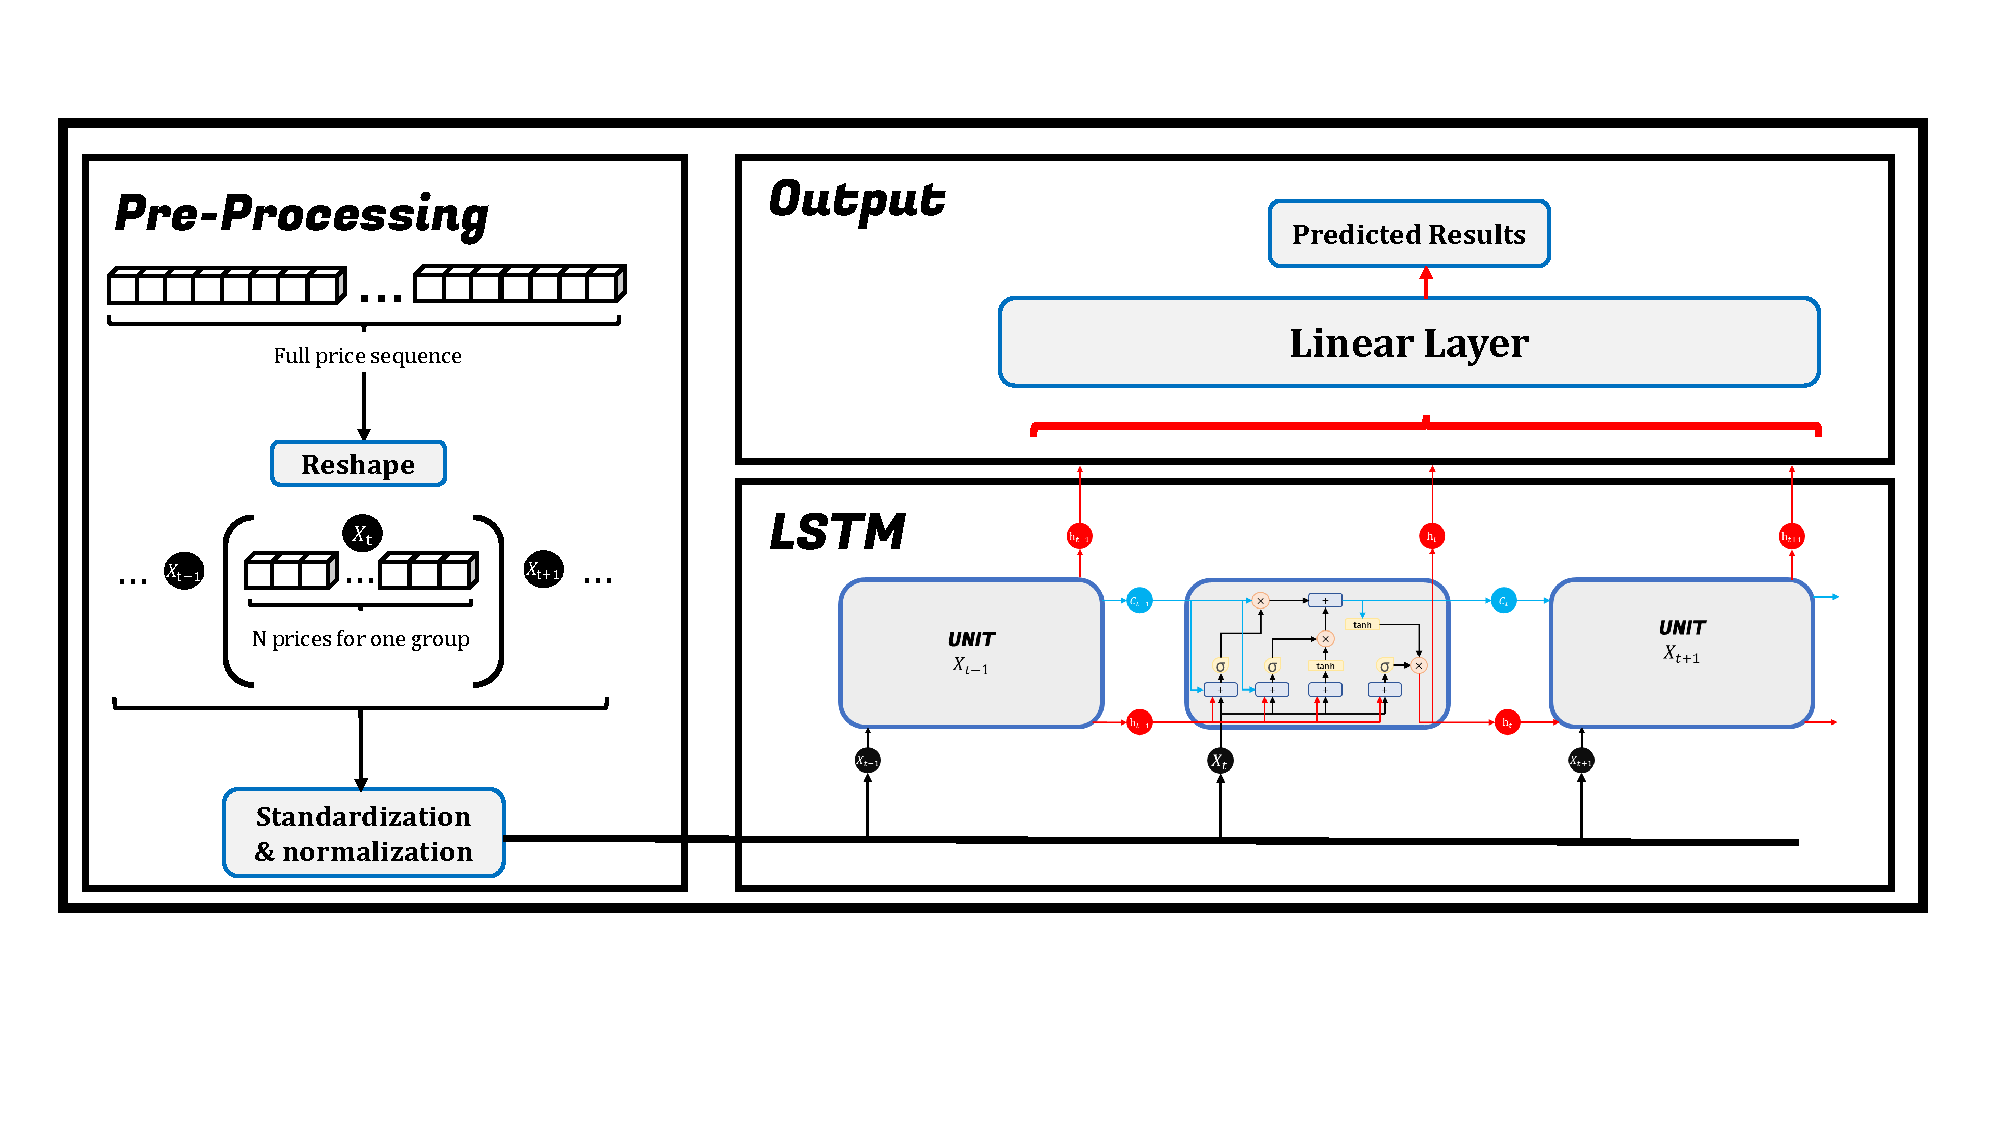
\includegraphics[width=0.9\textwidth]{LSTM_Fig}	%指定相同图片宽度,等比缩放
	\caption{Process of price forecasting} \label{fig:LSTM_model}		%题注、引用
\end{figure}
1. \textbf{Data Pre-processing}

When generating the data needed to predict the price of a particular day, one point to keep in mind is that the dataset we utilize is obtained only from prices before that day; this portion of the price series is referred to as the original price series. Before the preprocessing operation, we remove the null values from the original price sequence. In the preprocessing section, we first reshape the original price series to conform to the requirements for training data format. The initial one-dimensional price series is restructured into a dataset with an N-dimensional vector X serving as the feature and a scalar Y serving as the label. X indicates the price data we selected for the previous N days, and Y represents the actual price of the day as a label. 

Following that, we apply the necessary normalization to the data to keep the various variables within a comparable range and to accelerate the model's convergence:
\begin{equation}
	x_{i}=\frac{x_{i}-\mu_{i}}{\sigma_{i}}	
\end{equation}

%经典三线表
\begin{table}[H]
	\caption{\textbf{Symbols used in the pre-processing process}}%标题
	\label{Nota_PrePro}
	\centering%把表居中
	\begin{tabular}{cc}%四个c代表该表一共四列,内容全部居中
		\toprule%第一道横线
		Notation&Definition \\
		\midrule%第二道横线 
		N&The length of the price series used for forecasting \\
		X&The price sequence of the previous N days, used as a N-dimensional feature \\
		Y&The real price on a particular day, used as a label in the dataset 	\\
		$x_{i}$& An element in the $i^{th}$ N-dimensional feature\\
		$\mu_{i}$&The mean of the $i^{th}$ feature	\\
		$\sigma_{i}$&The standard deviation of the $i^{th}$ feature \\
		\bottomrule%第三道横线
	\end{tabular}
\end{table}


2. \textbf{LSTM Model}

Fig.\ref{fig:LSTM_unit} depicts the workflow of an LSTM unit.
\begin{figure}[H]	%浮动体参数
	\centering
	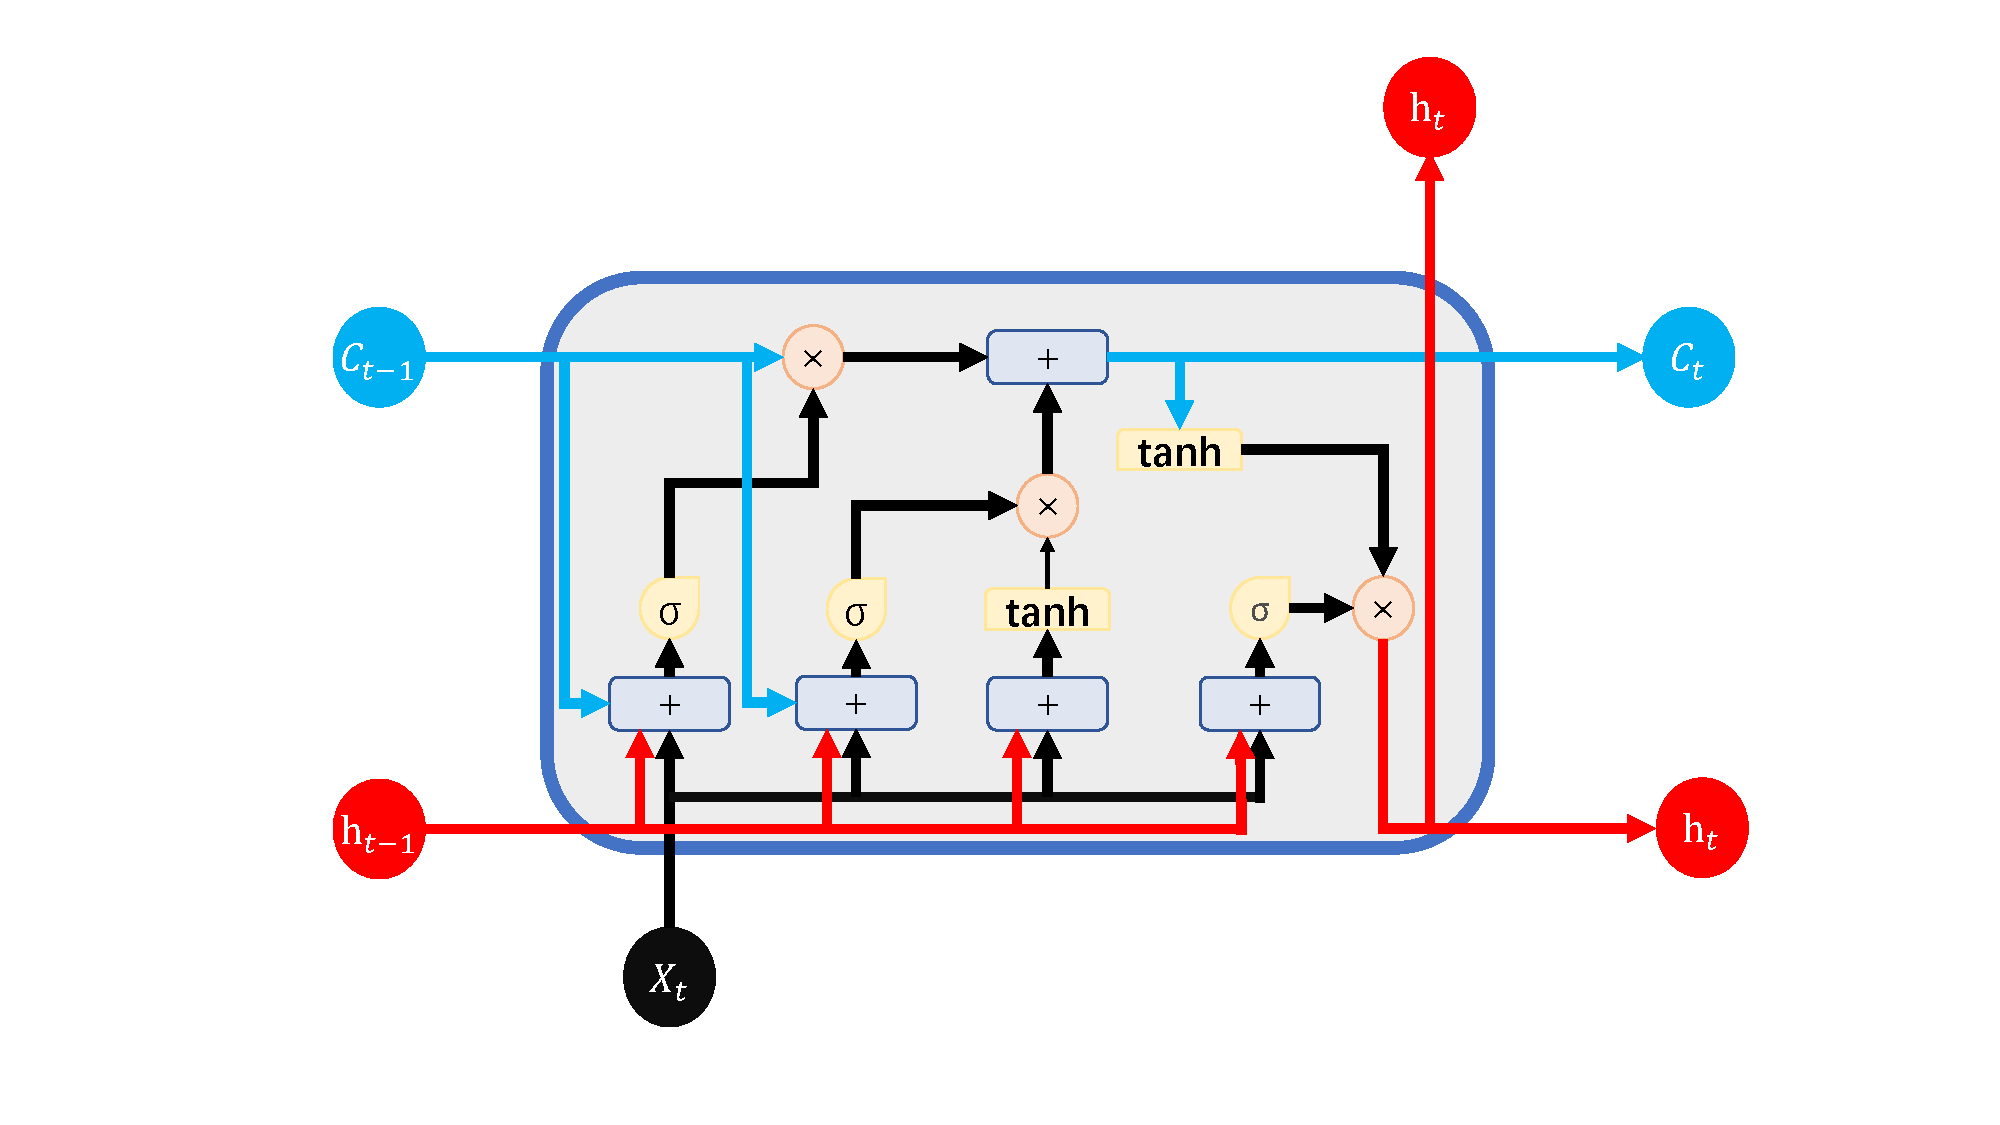
\includegraphics[width=0.8\textwidth]{LSTM_Unit}	%指定相同图片宽度,等比缩放
	\caption{Workflow of a single LSTM unit} \label{fig:LSTM_unit}		%题注、引用
\end{figure}
A series of actions will be carried out in this cell in order to produce the ultimate result:
\begin{equation}
	\left\{
	\begin{array}{lr}
		i_{t}=\mathrm{\sigma}\left( W_{ii}x_{t}+b_{ii}+W_{hi}h_{t-1}+b_{hi} \right) \,\, , &  \\
			f_{t}=\mathrm{\sigma}\left( W_{if}x_{t}+b_{if}+W_{hf}h_{t-1}+b_{hf} \right) \,\,, &	\\
		g_{t}=\tanh \left( W_{ig}x_{t}+b_{ig}+W_{hg}h_{t-1}+b_{hg} \right) , &  \\
		o_{t}=\mathrm{\sigma}\left( W_{io}x_{t}+b_{io}+W_{ho}h_{t-1}+b_{ho} \right) \,\, , &	\\
		c_{t}=f_{t}*c_{t-1}+i_{t}*g_{t} , & 	\\
		h_{t}=o_{t}*\tanh \left(c_{t} \right) , &
	\end{array}
	\right.
\end{equation}

The notations for equations above is shown in Table \ref{Nota_LSTM}:
%经典三线表
\begin{table}[H]
	\caption{\textbf{Symbols for a single LSTM cell}}%标题
	\label{Nota_LSTM}
	\centering%把表居中
	\begin{tabular}{cc}%四个c代表该表一共四列,内容全部居中
		\toprule%第一道横线
		Notation&Definition \\
		\midrule%第二道横线 
		$\mathrm{X}_{\mathrm{t}}$&The price series for the N days preceding the time t, used as the input vector for LSTM \\
		c&Memory cell, acting as an accumulator of the state information \\
		h&Hidden state, containing encoded information for the sequence flow	\\
		i&Input gate, controling whether the cell can acquire new input information\\
		f&Forget gate, controlling whether the past cell status could be “forgotten” in this process	\\
		o&Output gate, controlling whether the latest cell output will be propagated to the final state  \\
		W&The weight matrix of each node	\\
		b&The bias of each node \\
		$\sigma$&The sigmoid function \\
		tanh&The hyperbolic tangent function	\\
		\bottomrule%第三道横线
	\end{tabular}
\end{table}

3. \textbf{Output}

The output module is implemented here using a single linear layer. It accepts the LSTM's hidden layer state as input 
and produces the associated forecasted price.

\subsection{Prediction Results}
1. \textbf{Experiment setup}

	During the model's training process, the following settings are used:
	\begin{itemize}
		\item N, the length of the input price sequence (input feature vector), is set to 5.
		\item The experiments are run for 30 epochs with the learning rate 1e-2 and Adam optimizer.
		\item Each minibatch contains 10 5-dimensional sequences.
		\item Every 30 days, the model is retrained to ensure it remains up to date.
	\end{itemize}

2. \textbf{Result}

After training, we fed the complete 5-year price series (gold and bitcoin) into the model for prediction 
and obtained daily price predictions, which are compared to the real price series in Fig.\ref{fig:predict}

\begin{figure}[H]
	\centering
	\subfigure[Gold price forecasting by LSTM model]
	{
		\begin{minipage}{7cm}
			\centering
			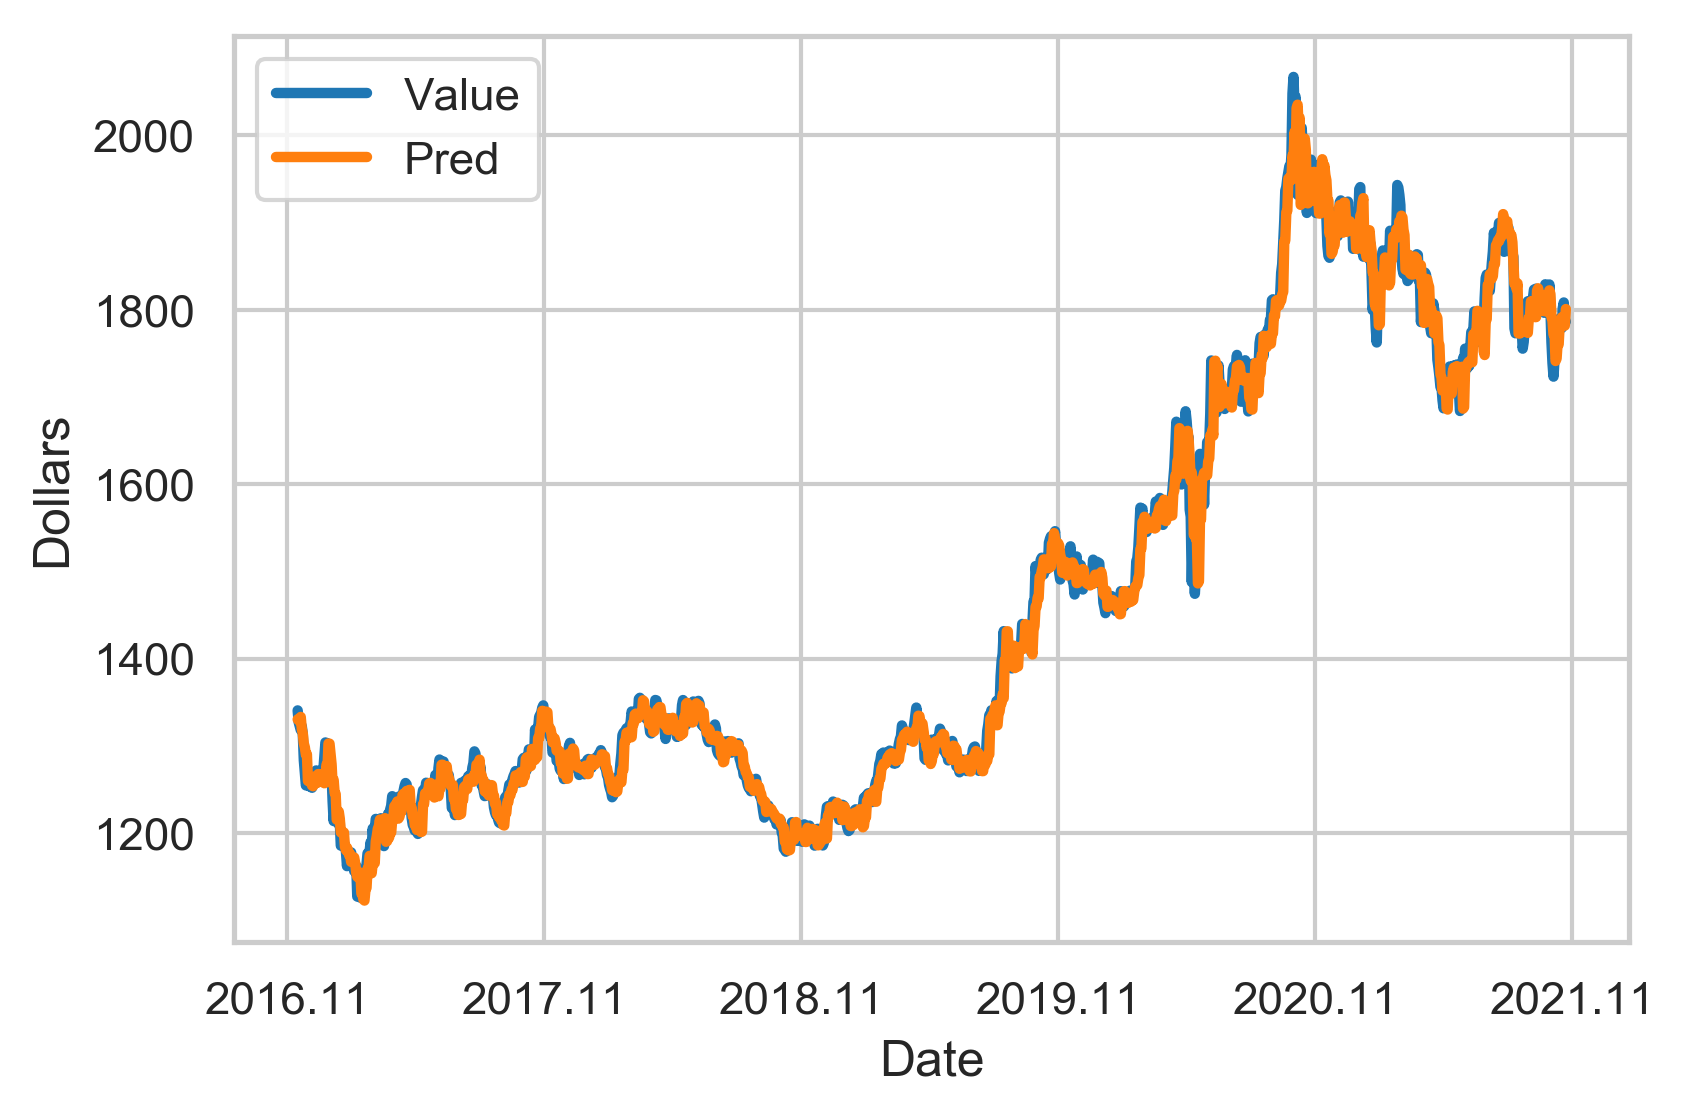
\includegraphics[scale=0.5]{lstm_gold}
		\end{minipage}
	}
	\subfigure[Bitcoin price forecasting by LSTM model]
	{
		\begin{minipage}{7cm}
			\centering
			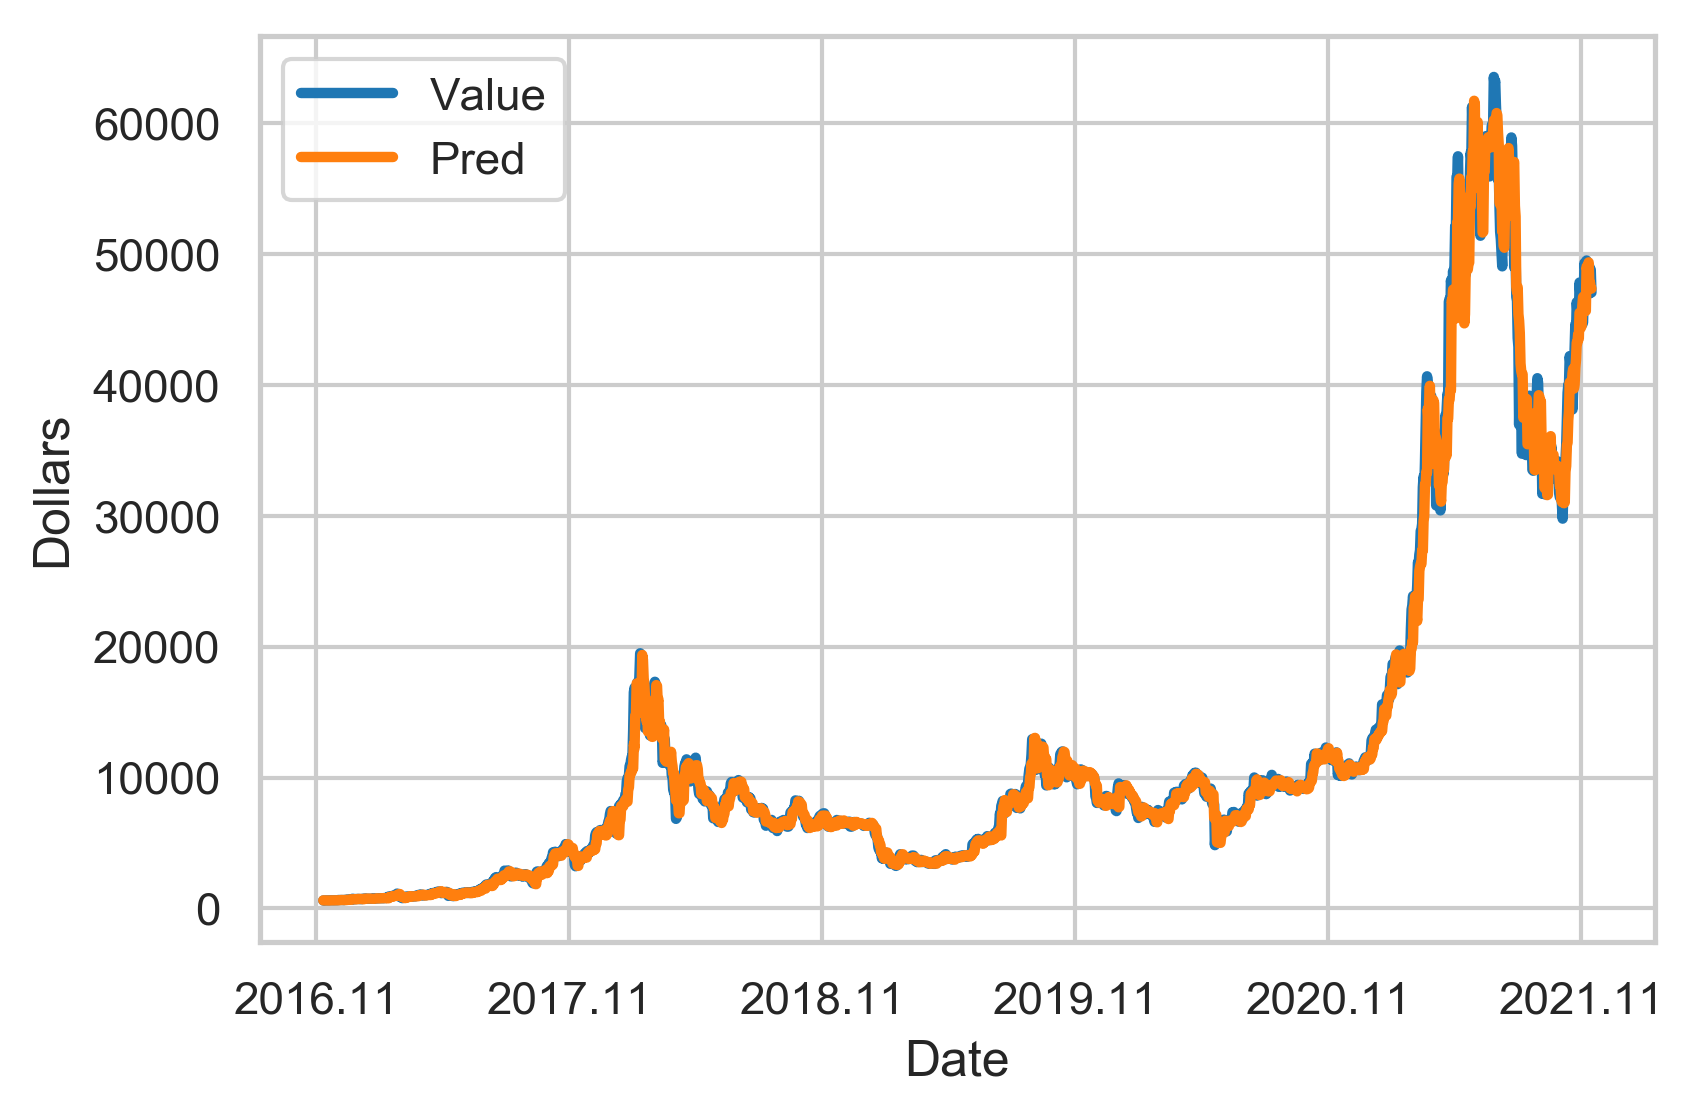
\includegraphics[scale=0.5]{lstm_bc}
		\end{minipage}
	}
	\caption{LSTM prediction results}
	\label{fig:predict}
\end{figure}

As illustrated in Fig.\ref{fig:predict}, forecasted prices can match and fit both gold and bitcoin's genuine values in terms of long-term trends and short-term variations. But there is a certain drawback to using this method for predicting early pricing (e.g., the first 30 days). It is worth noting that the sparse training data used to predict upfront prices results in somewhat unstable upfront prediction results. As a result, when developing the subsequent trading strategy, we will account for this effect and adopt a more cautious investment strategy in the early stages to mitigate its influence.

\subsection{Price Forecasting Model Evaluation}
In addition to the LSTM model, we applied several machine learning regression algorithms, including RanomForestRegressor, and eXtreme Gradient Boosting(xgboost) to forecast single-day price movements. We use metrics including Mean Square Error(MSE), Mean Absolute Error(RMSE), Root Mean Square Error(MAE), Mean Absolute Percentage Error (MAPE), coefficient of determination($R^{2}$)to measure the accuracy of these forecasting models, defined as follows:

\begin{equation}
MSE=\frac{1}{n} \sum_{i=1}^{n}\left(\hat{y}_{i}-y_{i}\right)^{2}
\end{equation}

\begin{equation}
RMSE=\sqrt{\frac{1}{n} \sum_{i=1}^{n}\left(\hat{y}_{i}-y_{i}\right)^{2}}
\end{equation}

\begin{equation}
MAE=\frac{1}{n} \sum_{i=1}^{n}\left|\hat{y}_{i}-y_{i}\right|
\end{equation}

\begin{equation}
	MAPE=\frac{100 \%}{n} \sum_{i=1}^{n}\left|\frac{\hat{y}_{i}-y_{i}}{y_{i}}\right|
\end{equation}

\begin{equation}
	R^{2}=1-\frac{\sum_{i}\left(\hat{y_{i}}-y_{i}\right)^{2}}{\sum_{i}\left(\overline{y_{i}}-y_{i}\right)^{2}}
\end{equation}
where $\hat{y}_{i}$ represents the predicted value, $y_{i}$ represents the true value, n represents the number of samples. These indicators measure the current error size, i.e. the smaller the value of the indicator, the higher the accuracy of the prediction model and the more reliable the prediction results. By substituting the anticipated values from the previously mentioned models for the genuine values, the following summary table of findings is generated:
%经典三线表
\begin{table}[H]
	\caption{\textbf{Error indicators for each model in predicting gold prices}}%标题
	\label{gold_pred_result}
	\centering%把表居中
	\begin{tabular}{cccccc}%四个c代表该表一共四列,内容全部居中
		\toprule%第一道横线
		Model&MSE&MAE&$R^{2}$&RMSE&MAPE \\
		\midrule%第二道横线 
		LSTM&\textbf{1534106.364}&\textbf{644.153}&0.992&\textbf{1238.590}&5.163\\
		LinearSVR&1896091.426&820.490&\textbf{0.994}&1376.986&\textbf{2.770}\\
		RanomForestRegressor&357287162.316&12441.370&-0.113&18902.041&28.602\\
		LightGBMRegressor&399364281.003&13310.400&-0.244&19984.100&30.865\\
		LinearRegression&1960022.9&853.448&0.993&1400.008&2.897 \\
		XGBoost&400260220.0&13338.557&-0.246&20006.504&31.107 \\
		\bottomrule%第三道横线
	\end{tabular}
\end{table}
%经典三线表
\begin{table}[H]
	\caption{\textbf{Error indicators for each model in predicting bitcoin prices}}%标题
	\label{bitcoin_pred_result}
	\centering%把表居中
	\begin{tabular}{cccccc}%四个c代表该表一共四列,内容全部居中
		\toprule%第一道横线
		Model&MSE&MAE&$R^{2}$&RMSE&MAPE \\
	\midrule%第二道横线 
		LSTM&\textbf{407.601}&\textbf{14.450}&\textbf{0.952}&\textbf{20.189}&\textbf{0.800}  \\
		LinearSVR&6877.521&17.101&0.889&82.930&1.107  \\
		RanomForestRegressor&45544.525&195.059&-4.293&213.411&10.555 	\\
		LightGBMRegressor&39998.423&180.965&-3.649&199.99&9.780 \\
		LinearRegression&409.262&14.622&0.952&20.230&0.809 \\
		XGBoost&61526.793&230.843&-6.151&248.045&12.522 \\
	\bottomrule%第三道横线
\end{tabular}
\end{table}
The bolded sections of the table represent the higher performing metrics, and you can see that the LSTM outperforms both gold and bitcoin prediction. So the aforesaid model will be used with the LSTM model in the subsequent trading strategy building. Due to the image scale's influence, the actual performance difference between different models is intuitively deduced from the graph, and we will evaluate these models using quantitative indicators throughout the subsequent actual trading process.


\begin{comment}
	\begin{figure}[H]
		\centering
		\subfigure[Gold price forecasting - using LightGBM algorithm]{
			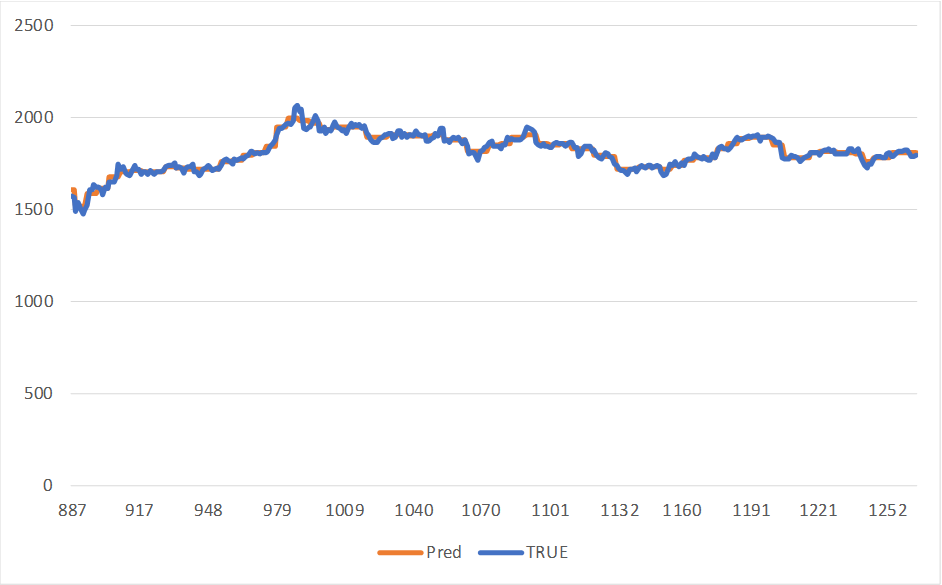
\includegraphics[width=5.5cm]{LightGBM_gold}
		}
		\quad
		\subfigure[Bitcoin price forecasting - using LightGBM algorithm]{
			\includegraphics[width=5.5cm]{LightGBM_bit}
		}
		\quad
		\subfigure[Gold price forecasting - using GBDT algorithm]{
			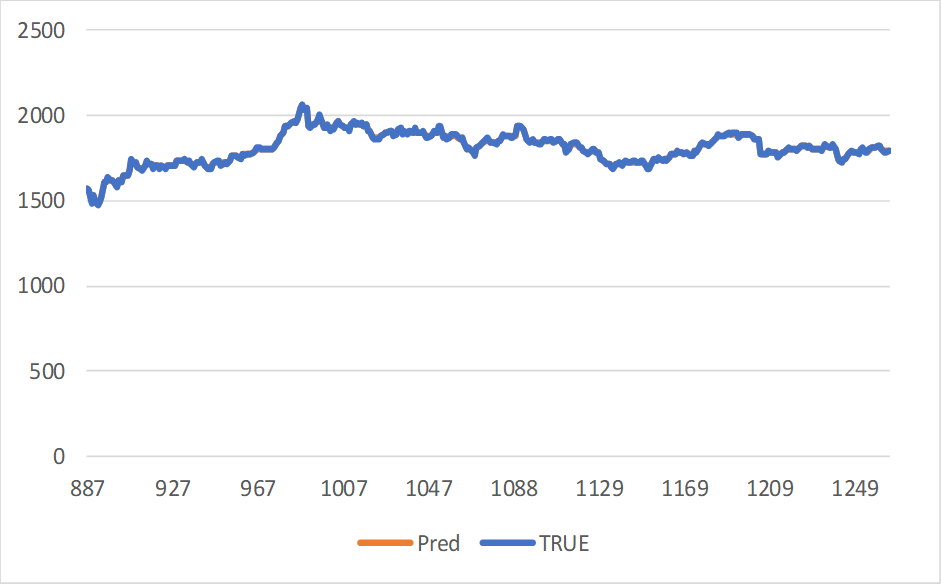
\includegraphics[width=5.5cm]{GBDT_gold}
		}
		\quad
		\subfigure[Bitcoin price forecasting - using GBDT algorithm]{
			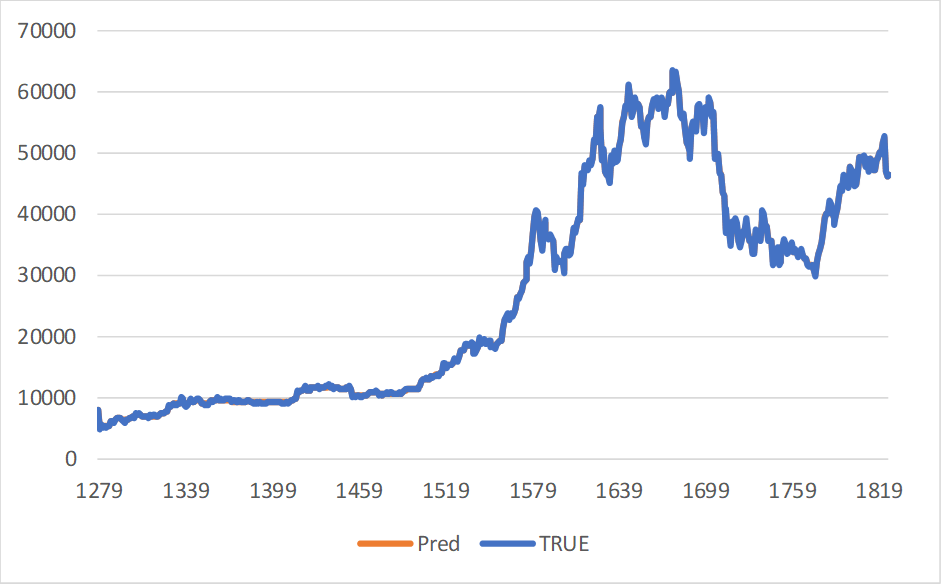
\includegraphics[width=5.5cm]{GBDT_bit}
		}
		\quad
		\subfigure[Gold price forecasting - using xgboost algorithm]{
			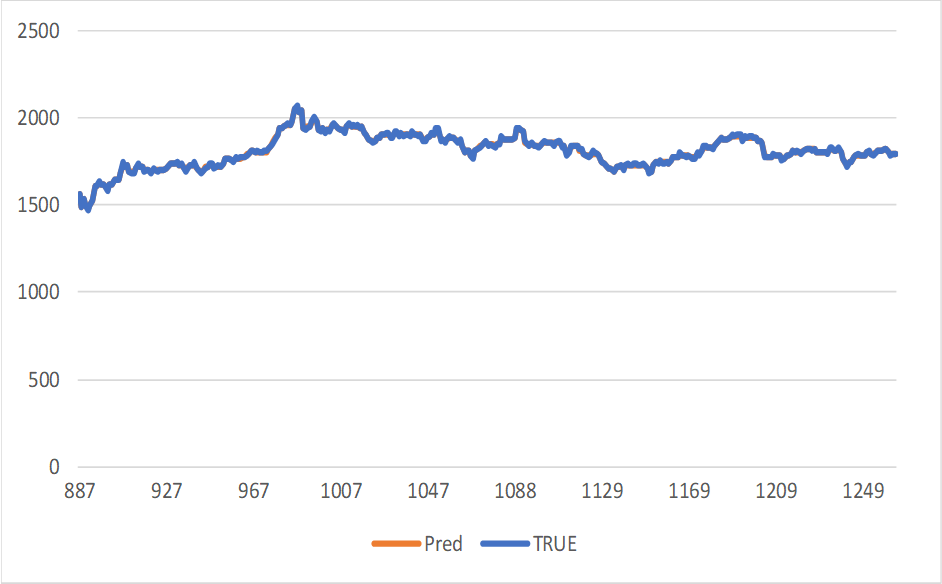
\includegraphics[width=5.5cm]{xgboost_gold}
		}
		\quad
		\subfigure[Bitcoin price forecasting - using xgboost algorithm]{
			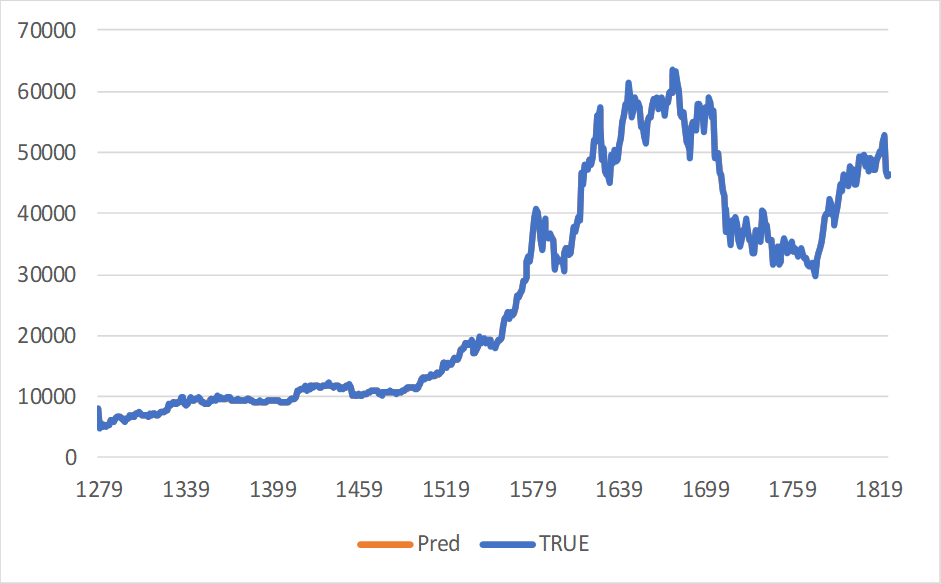
\includegraphics[width=5.5cm]{xgboost_bit}
		}
		\caption{Predicted price curves of other models}
		\label{fig:other_model_predict}
	\end{figure}内容...
\end{comment}


\section{Model 2: Quantitative Trading}
\subsection{Model Overview}
Quantitative trading is a type of trading approach in which a large amount of investment-related data is used as a sample to develop quantitative mathematical models and formulas, estimate the probability of various market movements, and programmatically execute buy and sell orders to achieve investment\cite{Quan1}.

Generally, quantitative trading strategies can be classified as the trending strategy and the market neutral strategy. The trend-following strategy is a very systematic approach with very specific rules: \textbf{purchase when an entry signal occurs and sell when an exit signal appears}. Price is the most important factor in a trend following strategy, while asset management and risk control are also very important components. Thus, a comprehensive trading strategy will often comprise the underlying's selection, entry and exit timing, position and capital management, and the risk control solution. Based on the trend-following strategy, we develop a quantitative trading method that is sensitive to market fluctuations and stable to risk.

Among the components of a trading strategy, the underlying asset for the trade has been specified in this question, which includes a more stable traditional asset (gold) and a riskier digital asset (bitcoin). As such, we will focus on creating our trading strategy on the following points:
\begin{itemize}
	\item Establishing the proper \textbf{entry and exit signals}
	\item Optimizing the \textbf{asset-to-asset allocation ratio}
	\item Constructing a tool for \textbf{precise positioning adjustment}
	\item Creating a workable \textbf{risk management systems}
\end{itemize}

In the post, we begin by introducing the key indicators that will be used and then describe the entire strategy in modules.

\subsection{Description of the Indicator}
1. \textbf{Average True Range (ATR)}

ATR is a volatility indicator that measures market volatility by decomposing the entire range of an asset price for that period\cite{ATR}. There are two steps in the calculation of the ATR: first, the true range (TR) of the asset is determined; and then a moving average (MA) is used to smooth the ATR:

$$
	\centering
	TR=\operatorname{Max}\left[(H-L), \operatorname{Abs}\left(H-C_{P}\right), \operatorname{Abs}\left(L-C_{P}\right)\right]  
$$
$$
	ATR=\left(\frac{1}{n}\right) \sum_{(i=1)}^{(n)} T R_{i}
$$

where H denotes the day's highest price, L denotes the day's lowest price, and $P_{t-1}$ denotes the previous day's price, and n denotes the time period used. 

Due to the fact that the daily price in the data provided in this question is a constant amount, — in other words, H equals L, refer as the day's price $P_{t}$. Therefore, the computation process can be streamlined as follows:
\begin{equation}
	ATR=\left(\frac{1}{n}\right) \sum_{i=1}^{n} (P_{t}-P_{t-1})
\end{equation}

2.  \textbf{Maximum Adverse Excursion(MAE) and Maximum Favorable Excursion(MFE)}

MAE indicates the low point of a long trade and the high point of a short trade. It assists in determining the trade's maximum loss. This is often referred to as the position's maximum drawdown. MFE indicates the high point of a long trade and the low point of a short trade. It shows the profit earned during a trade. The calculation steps for these two indicators are as follows:
\begin{gather}
	\mathrm{MFE}=\left(\frac{1}{n}\right)\left(\sum_{1}^{n} \operatorname{Abs}(P_{i}-P_{iL}) / ATR\right) \\
\mathrm{MAE}=\left(\frac{1}{n}\right)\left(\sum_{1}^{n} \operatorname{Abs}(P_{i}-P_{iH}) / ATR\right) 
\end{gather}
where $n$ represents the total times of market entry signals, $P_{i}$ represents the price of the $i^{th}$ transaction, and $P_{iH}$ and $P_{iL}$ represent the maximum and minimum price in the calculation period.

Based on the MAE and MFE, we can get a plausible signal for market entry: E-ratio. The following is the definition:
\begin{equation}
	\mathrm{E_{ratio}}=\frac{MFE}{MAE}\\
\end{equation}

3. \textbf{Sharpe Ratio}

The Sharpe ratio is used to help investors understand the return of an investment compared to its risk. When comparing two assets, the one with a higher Sharpe ratio appears to provide better return for the same risk, which is usually attractive to traders\cite{sharpe}. It is a crucial factor for risk evaluation in our trading techniques and is defined as follows:
\begin{equation}
	S_{a}=\frac{E\left[R_{a}-R_{b}\right]}{\sigma_{a}}=\frac{E\left[R_{a}-R_{b}\right]}{\sqrt{\operatorname{var}\left[R_{a}-R_{b}\right]}}
\end{equation}
where $R_{a}$ is the asset return, $R_{b}$ is the risk-free return. $E[R_{a}-R_{b}]$ is the expected value of the excess of the asset return over the benchmark return, and $\sigma _{a}$ is the standard deviation of the asset excess return.

\subsection{Model Structure}
The basic flow of our trading strategy is shown in Fig.\ref{fig:trade}
\begin{figure}[H]	%浮动体参数
	\centering
	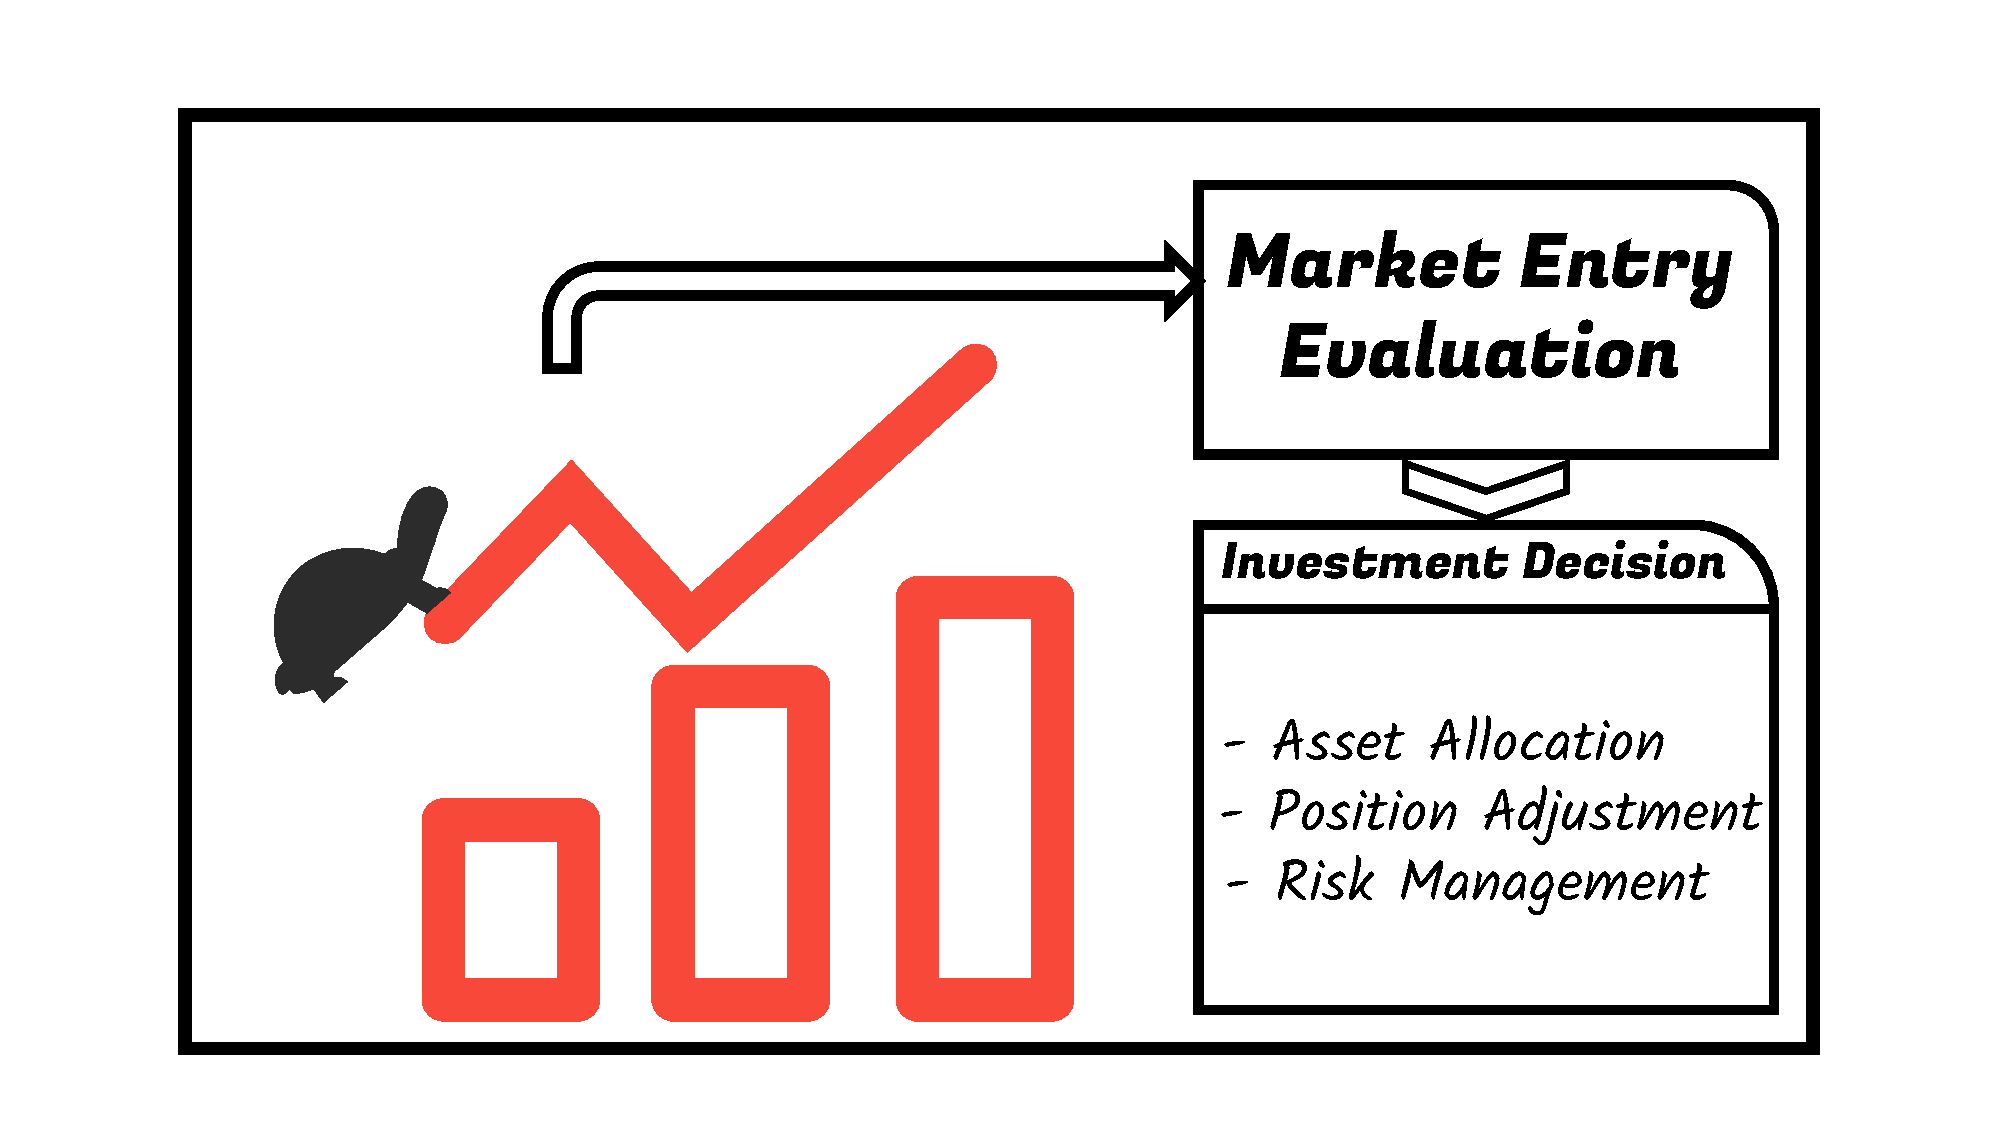
\includegraphics[height=0.4\textwidth]{trade}	%指定相同图片宽度,等比缩放
	\caption{Structure of the trading model} \label{fig:trade}		%题注、引用
\end{figure}
The initial step is to evaluate current market conditions and then enter the market for investment after those conditions are met. The following phase will be to establish the fairest investment ratio and allocation ratio for the two assets using a series of judgment procedures and optimization techniques to ensure that return and risk are balanced. We will outline the approach and important judgment indicators in chronological order, beginning with market entry and ending with investment.

1. \textbf{Market Entry Evaluation}

In the forecasting section we have mentioned that due to the small number of price datasets corresponding to the first 30 days, there are large fluctuations and deviations in the forecast values. As a result, entering the market during the early stages is a dangerous and ill-advised action. We choose to evaluate the entry signal after 30 days.

The E-ratio is a frequently utilized market entrance indicator. We update it on a 10-day cycle for gold and bitcoin. When the E-ratio exceeds 1.4, we consider it a strong entry signal and choose to enter the market by withdrawing a certain percentage of cash in hand to purchase bitcoin/gold to begin the investing adventure; the percentage of money used for the entry is an arbitrarily chosen hyperparameter.

2. \textbf{Basic conditions and guidelines}

The basic concept of investing is to \textbf{buy today for future gains when the price is projected to climb tomorrow} and to \textbf{sell today for a stop loss when the price is predicted to fall tomorrow}. Specifically for purchase operations, buying is only authorized if the buy return is greater than the hold return. This condition can be represented as follows:



\begin{align}
	\left\{\begin{array}{l}
		x+n_{1g}m_{2g}<x-1.01(n_{2g}-n_{1g})m_{1g}+m_{2g}n_{2g} \\
		x+n_{1b}m_{2b}<x-1.02(n_{2b}-n_{1b})m_{1b}+m_{2b}n_{2b}
	\end{array}
	\right. \Rightarrow
	\left\{\begin{array}{l}
		m_{2g}>1.01 m_{1g} \\
		m_{2b}>1.02 m_{1b}
	\end{array}\right.
	\label{earn_condition}
\end{align}
Selling is the same , We only sell if the sell loss is less than hold loss .The conditions are as follows:  
\begin{align}
\left\{\begin{array}{l}
x+n_{1g}m_{2g}>x+0.99(n_{2g}-n_{1g})m_{1g}+m_{2g}n_{2g} \\
x+n_{1b}m_{2b}>x+0.98(n_{2b}-n_{1b})m_{1b}+m_{2b}n_{2b}
\end{array}
\right. \Rightarrow
\left\{\begin{array}{l}
m_{2g}<0.99 m_{1g} \\
m_{2b}<0.98 m_{1b}
\end{array}\right.
\label{earn_condition}
\end{align}


where $x$ represents cash held this day, $n_{1}$ represents the number of assets held this day, $n_{2}$ represents the number of assets held tomorrow, $m_{1}$ represents the unit price of the asset today, and $m_{2}$ represents the unit price of the asset tomorrow. The subscript $b$ means bitcoin and the subscript $g$ means gold, with different trading commissions. These two inequalities, which apply to the acquisition of gold and bitcoin, will be referred to as $\boldsymbol Condition 1$ and  $\boldsymbol Condition 2$, respectively.


3. \textbf{Investment Decision}

Table \ref{Nota_invest} summarizes the parameters utilized in the investment decision-making process.
%经典三线表
\begin{table}[H]
	\caption{\textbf{Symbols for the trading strategy}}%标题
	\label{Nota_invest}
	\centering%把表居中
	\begin{tabular}{cc}%四个c代表该表一共四列,内容全部居中
		\toprule%第一道横线
		Notation&Definition \\
		\midrule%第二道横线 
		$C$&The amount of cash held on the day (in U.S. dollars)\\
		$G$&The amount of gold held on the day (in ounces)\\
		$B$&The amount of bitcoin held on the day \\
		$P_{g}$&The price of gold per ounce on the day\\
		$P_{b}$&The price per bitcoin on the day\\
	    $\nu$&The total value of the current portfolio \\
		$\tau$&The risk volatility of a portfolio \\
		$\gamma$&The daily rate of return on a portfolio\\
		$s$&The Sharpe Ratio\\
		$I_{f}$&The Investment factor\\
		\bottomrule%第三道横线
	\end{tabular}
\end{table}
Given the fact that gold has a trading day limit, we need to verify the current day before trading, and the results fall into two categories:
\begin{enumerate}[fullwidth,itemindent=2em,label=\roman*.]
	\item If the day is not a gold trading day, the trade will be limited to bitcoin.
			Purchase bitcoin when the estimated bitcoin price for tomorrow meets $\boldsymbol Condition 1$ from equation(\ref{earn_condition}), the exact percentage of this purchase is calculated below.
	\item While a gold trading day occurs, take into account both the rise and fall of gold and bitcoin when determining the ideal investment configuration.
\end{enumerate}

Following that, we ascertain the precise quantity and percentage of investment. Take note that we are addressing a hypothetical situation here; the scenario in which only bitcoins can be traded is a simplification of this scenario. To begin, we assume that the portfolio holdings for today are $[C1,G1,B1]$, those for tomorrow are $[C2,G2,B2]$, and the total value of the current portfolio are:
\begin{equation}
	\nu= C + G \times  P_{g} + B \times P_{b} \\
\end{equation}

From the above formula, the total value of assets today and total value of assets tomorrow are indicated as $\nu_{1}$ and $\nu_{2}$ correspondingly.

Then the rate of return of this investment is:
\begin{equation}
	\gamma =\left(\nu _{2}-\nu_{1}\right) / \nu_{1}\\
\end{equation}

Presuming no extra return on cash holdings, we define the risk volatility of the portfolio for tomorrow as follows:
\begin{equation}
\tau =\sqrt{\left(G \times P_{g-total} \times S_{td_{1}}\right)^{2}+\left(B \times P_{b-total} \times S_{td_{2}}\right)^{2}}\\
\end{equation}

where $P_{g-total}$ refers to the total value of gold held on tomorrow, $P_{b-total}$ refers to the total price of bitcoin held on tomorrow, $S_{td_{1}}$ refers to the standard deviation of the price of gold in the last month, and $S_{td_{2}}$ refers to the standard deviation of the price of gold in the last month.

The Sharpe ratio for this portfolio is:
\begin{equation}
	s=\frac{\gamma -R_{f}}{\tau }
\end{equation}

where $R_{f}$ is the risk-free return, which is assumed to be $0$ here.

By combining the aforementioned parameters, we create a metric called the \textbf{Investment Factor} that reflects a composite representation of return and risk.It is defined as follows:
\begin{equation}
	I_{f}= \alpha \cdot \gamma +\beta \cdot S 
\end{equation}

where $\alpha$ is the ratio of daily return rate to investment factor, and $\beta$ is the ratio of daily Sharpe Ratio to investment factor. They are two hyperparameters that have been artificially established.
We can infer that investment factor $I_{f}$ possesses the following two properties:
\begin{itemize}
	\item Directly proportional to the rate of return, i.e. the higher the rate of return, the greater the investment factor $I_{f}$
	\item Inversely proportional to the risk, i.e. the smaller the risk, the greater the investment factor $I_{f}$
\end{itemize}

From the above, we can maximize the investment factor $I_{f}$ by optimizing the portfolio $[C2,G2,B2]$, thereby obtaining the optimal portfolio with a relatively high rate of return and a low rate of risk.

By changing the size of $\alpha$  and $\beta$, investors with different degrees of aggressiveness can be simulated: if one is an aggressive investor who only values returns and does not count risks, one can set $\alpha$  to be larger and $\beta$ to be smaller, while if one is a conservative investor who favors less risky investments, one can set $\beta$ to be larger.

\subsection{Model Optimization and Solution}

According to the above description of the investment factor, we can deduce that the investment factor $I_{f}$ is only related to the portfolio $[C2,G2,B2]$, and that portfolio satisfies the following constraint relationship:
\begin{equation}
C_{1}+G_{1} \times P_{g_{1}}+B_{1} \times P_{b_{1}}=C_{2}+G_{2} \times P_{g_{1}}+B_{2} \times P_{b_{1}} - M 
\end{equation}

Where M is the fee required for this transaction, which is calculated as:
\begin{equation}
M = 0.01\times(G_{2} - G_{1}) \times P_{g_{1}}+0.02 \times (B_{2} - B_{1}) \times P_{b_{1}}
\end{equation}

So we can use the PSO(Particle swarm optimization), change different portfolios, and perform fast iterative optimization to obtain the maximum investment factor, the specific algorithm process of the pseudo code is as follows:

\begin{algorithm} [H]
	\caption{Maximize $I_{f}$} 
	\label{alg3} 
	\begin{algorithmic}
		\FOR{each particle $i$}
		\STATE{Initialize velocity $V_{i}$ and position $X_{i}$ for particle $i$\\
		Evaluate particle $i$ and set $pBesti = X_{i}$} 
		\ENDFOR\\
		$IBest = max(pBesti)$\\
		\WHILE{not stop}
		\FOR{$i = 1 to N$}
		\STATE{Update the velocity and position of particle i\\
		Evaluate particle i} 
		\IF{$fit(X_{i}) <  fit(pBesti)$}
		\STATE $pBesti = X_{i}$
		\ENDIF
		\IF{$fit(pBesti) < fit(IBest) $}
		\STATE $IBest = pBesti$
		\ENDIF
		\ENDFOR
		\ENDWHILE
		\\$I_{f} = IBest$
	\end{algorithmic} 
\end{algorithm}

Finally, using our model and strategy, the initial \textbf{1,000 \$} becomes \textbf{108,387.309 \$} after five years


\section{Model Evaluation}
To prove that our model gives the best trading strategy, we must assess a variety of investment models and objectively compare their strengths and flaws to show that ours is the best. To that purpose, we go through three metrics that are frequently used to assess quantitative trading: APR(Annual Percentage Rate),SharpeRatio, MD(Maximum drawdown).

Based on these quantitative metrics, we compare our model with several traditional quantitative investment models to demonstrate that our model offers the best trading strategy.The results obtained are shown in the following table:

%经典三线表
\begin{table}[H]
	\caption{\textbf{Model evaluation results}}%标s题
	\label{Model Evaluation}
	\centering%把表居中
	\begin{tabular}{cccc}%四个c代表该表一共四列,内容全部居中
		\toprule%第一道横线
		Model&APR&Sharpe Ratio&MD \\
	\midrule%第二道横线 
	Our Model&1.296&1.28&0.38\\
	CAPM Model&1.15&1.07&0.51\\
	MDP Model&1.05&1.21&0.31\\
	Maekowitz Model&1.37&0.78&0.63\\
	\bottomrule%第三道横线
\end{tabular}
\end{table}
%经典三线表

The above table is created in the style of a radar chart to help you see the benefits of our model more clearly.

\begin{figure}[H]	%浮动体参数
	\centering
	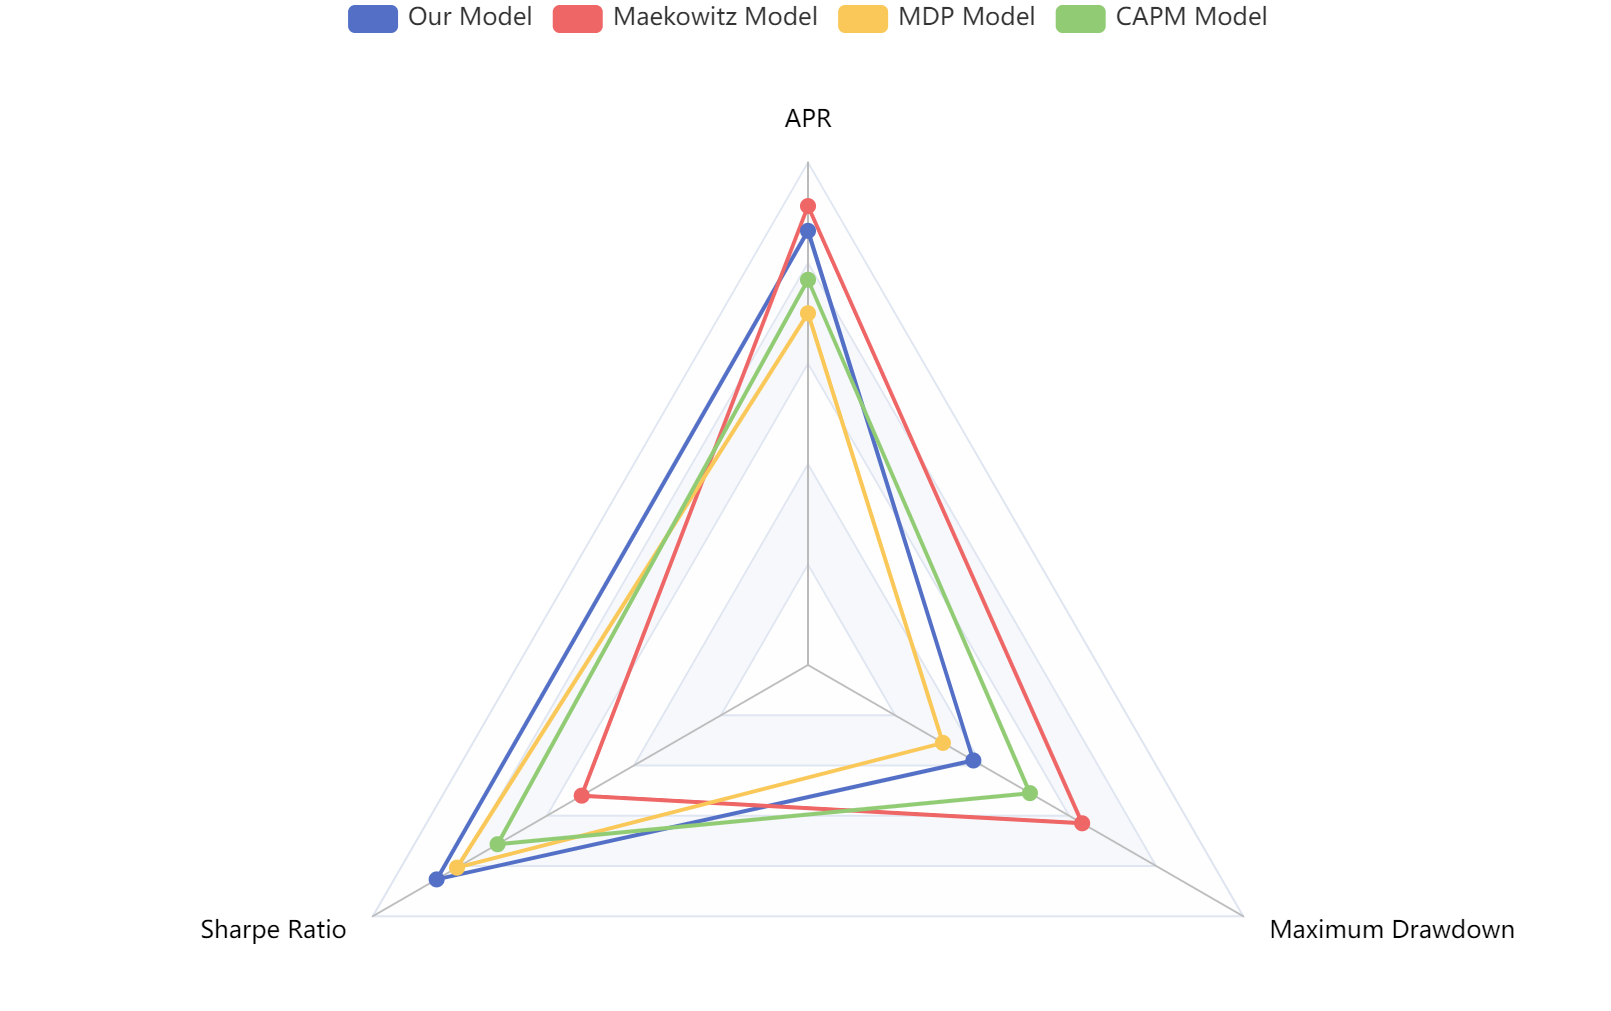
\includegraphics[height=0.6\textwidth]{radar}	%指定相同图片宽度,等比缩放
	\caption{Radar plot of model evaluation results} 
	\label{fig:radar}		%题注、引用
\end{figure}

Compared with other models , our decision model has the highest APR and Sharpe ratio, and the 30-day maximum retracement is below 40\%, as shown in the Figure 5, indicating that our model has the highest return with managed risk and can prove that our model provides the best strategy.


\newpage
\section{Sensitivity Analysis}
\subsection{Value Sensitivity}
Two main parameters are subjected to sensitivity analysis: $\alpha_{gold}$ (Commissions on gold transactions) and $\alpha_{bitcoin}$ (Commissions on bitcoin transactions). First, we change the value of $\alpha_{gold}$ from 0.2\% to 1.8\%, with each step increasing by 0.4\%. The results, as shown in Figure 5(a), show that the trend in the overall value of the portfolio only varies significantly. Then, similarly, we change the value of $\alpha_{bitcoin}$ from 1\% to 3\%, with each step increasing by 0.5\%, and evaluate its sensitivity. It does not appear to be notably sensitive,except after 2015, as illustrated in Figure 5(b). Finally, we modify the values of $\alpha_{gold}$ and $\alpha_{bitcoin}$ at the same time to see how the trend changes. It can be found in Figure 5(c) that even when changing the commission ratio for both gold and bitcoin, the total value of the portfolio generated by our model remains within a tolerable range, demonstrating good robustness and insensitivity to commission changes.



\begin{figure}[H]
	\centering
	\subfigure[Only $\alpha_{gold}$]{
		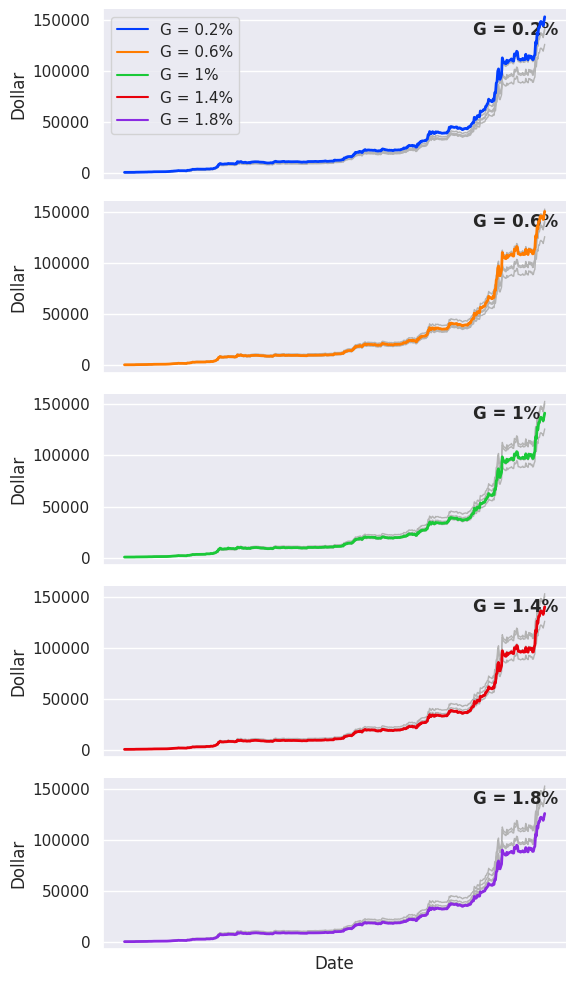
\includegraphics[width=5cm]{gold_sensitivity}
		%\caption{fig1}
	}
	\quad
	\subfigure[Only $\alpha_{bitcoin}$]{
		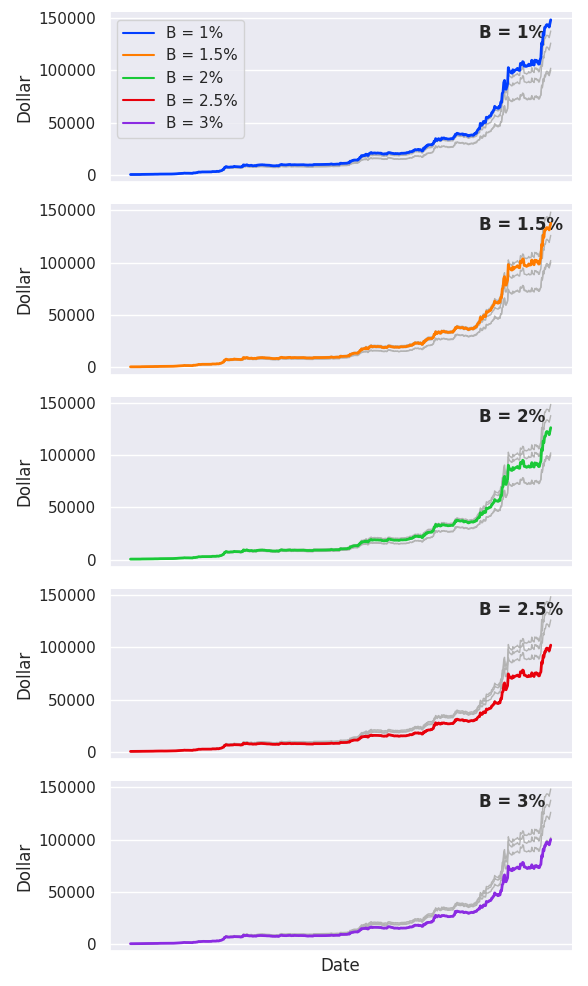
\includegraphics[width=5cm]{bc_sensitivity}
	}
	\subfigure[$\alpha_{gold}$ and $\alpha_{bitcoin}$]{
		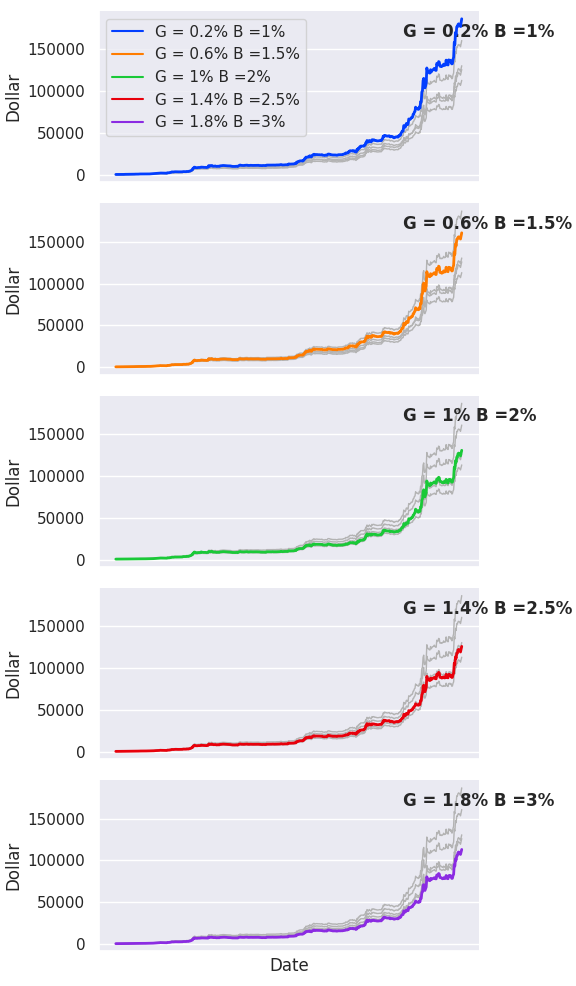
\includegraphics[width=5cm]{gold_bc_sensitivity}
	}
	\caption{Value Sensitivity}
	%\label{fig:bc_sensitivity}		%题注、引用
\end{figure}
\newpage
\subsection{Asset Ratio Sensitivity}
We examine the influence of different commission percentages on asset ratios by adjusting the values of a and b and examining the respective percentages of cash, gold, and bitcoin in the final portfolio

\begin{figure}[H]
	\centering
	\subfigure[ $\alpha_{bitcoin}$=1.5\%,$\alpha_{gold}$=1\%]{
		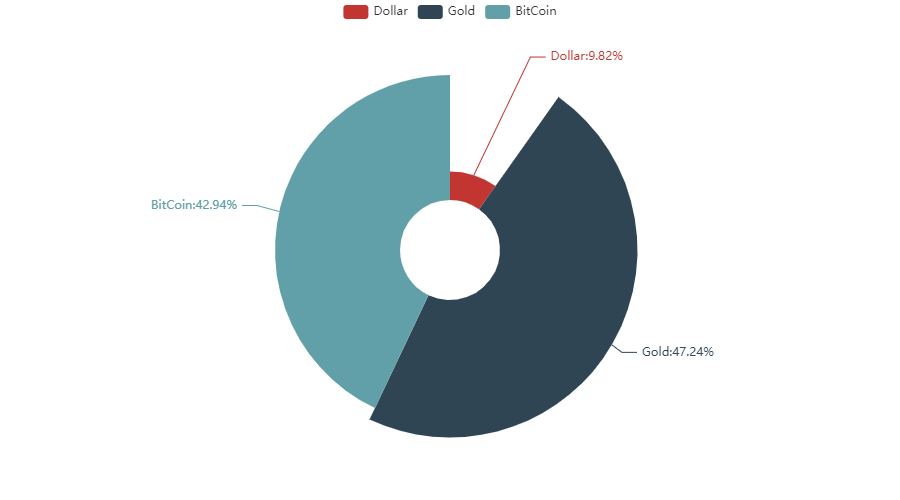
\includegraphics[width=5.5cm]{b=1.5,g=1}
		%\caption{fig1}
	}
	\quad
	\subfigure[ $\alpha_{bitcoin}$=2.5\%,$\alpha_{gold}$=1\%]{
		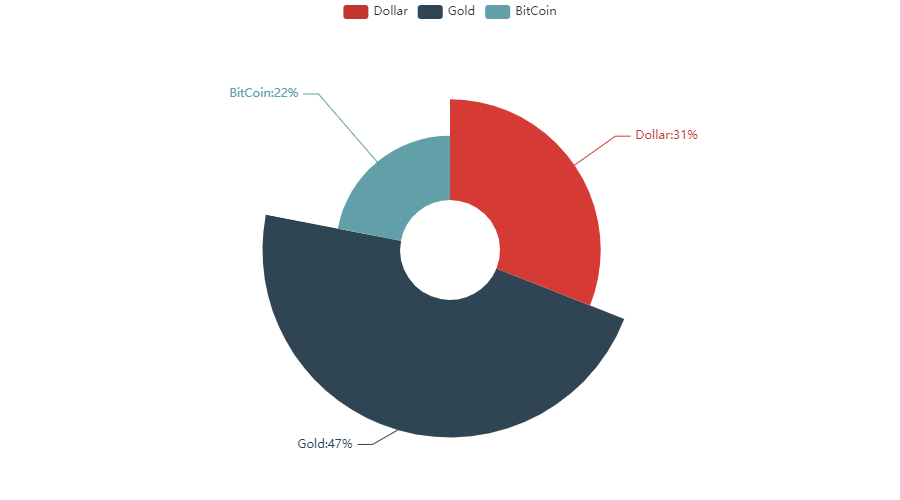
\includegraphics[width=5.5cm]{b=2.5,g=1}
	}
	\quad
	\subfigure[ $\alpha_{bitcoin}$=2\%,$\alpha_{gold}$=1\%]{
		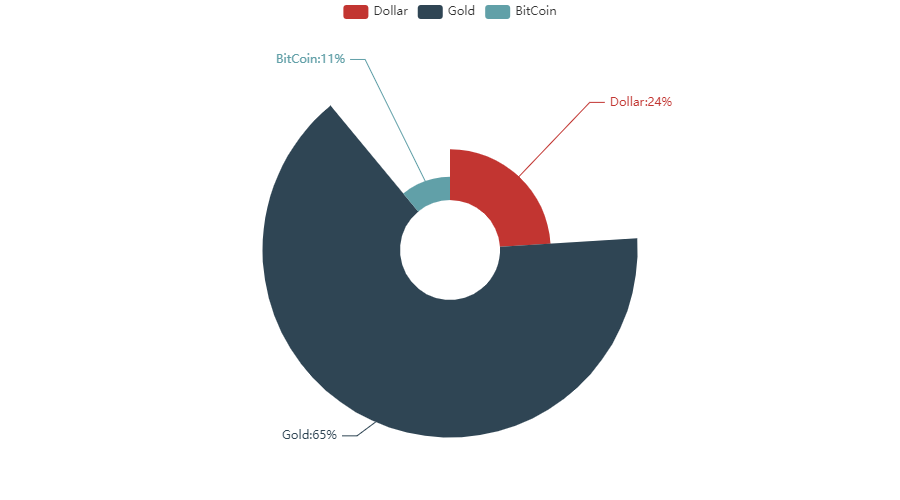
\includegraphics[width=5.5cm]{b=2,g=1}
	}
	\quad
	\subfigure[ $\alpha_{bitcoin}$=2\%,$\alpha_{gold}$=0.5\%]{
		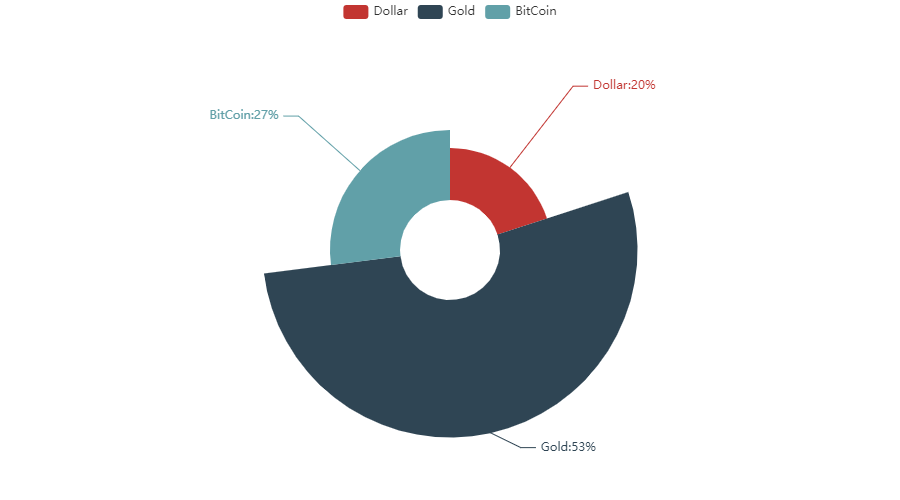
\includegraphics[width=5.5cm]{b=2,g=0.5}
	}
	\quad
	\subfigure[ $\alpha_{bitcoin}$=2\%,$\alpha_{gold}$=1.5\%]{
		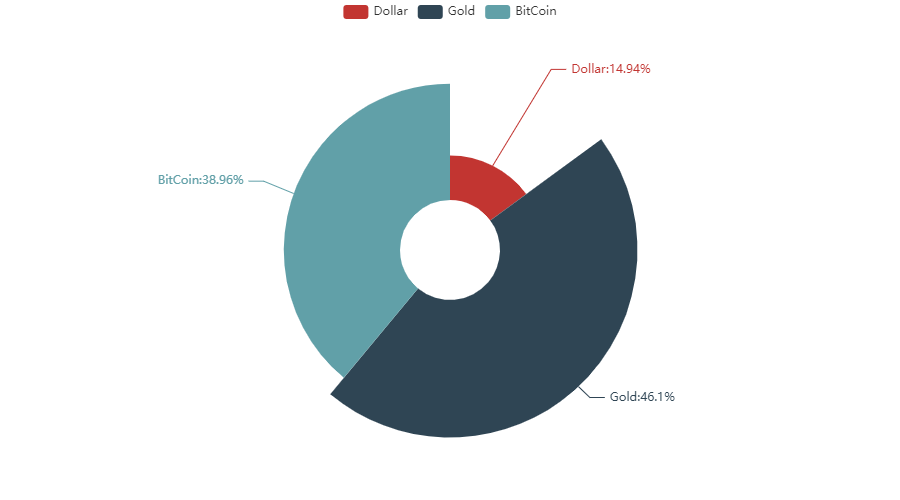
\includegraphics[width=5.5cm]{b=2,g=1.5}
	}
	\caption{Value Sensitivity}
	%\label{fig:bc_sensitivity}		%题注、引用
\end{figure}

As you can see from these asset share distribution charts, the percentage of bitcoin holdings increases slightly when bitcoin commissions fall and decreases slightly when bitcoin commissions rise, ditto for gold. This is in line with the basic market rule


\section{Strengths and Weaknesses}
\subsection{Strengths}
\begin{enumerate}
	\item In the price forecast section, we combine short-term price fluctuations and long-term pricing patterns and anticipate future prices using a variety of models, including LSTM, random forest, and others. To assure the process's integrity and reliability, these forecasting approaches are reviewed using a range of quantitative indicators and graphical analyses.
	\item In the investment decision section, we develop a comprehensive market entry strategy based on the ATR, MAE, MFE, and E-ratio, and designed the investment factor as an indicator to evaluate the trading upsides and downsides by integrating the price trend, return rate, and risk appetite. Thus, determining trading strategies boils down to an optimization problem in which alternate hyperparameters can modify the model's long-term tendency, enhancing the model's ultimate outcome while increasing the strategy's customizability and interpretability.
	\item In the strategy evaluation section, we evaluate and compare different strategies in multiple dimensions such as return, stability, risk, maximum retracement, etc. We provide a comprehensive description of the performance differences between the models horizontally and systematically explain the model's unique benefits and justifications for these advantages.
	\item In the sensitivity analysis section, we examine the impact of varying commission ratios on the model's results on total assets. Additionally, we monitor daily fluctuations in the trading volume of each asset class to demonstrate the impact of commission changes on the strategy preferences and allocation ratio of the two assets, as well as to demonstrate the complete strategy modifications in each asset.
\end{enumerate}

\subsection{Weaknesses}
\begin{enumerate}
	\item The accuracy of the price prediction findings is limited because the data given in the question does not include additional information, such as the opening price, closing price, trading volume, etc. This has an impact on the assessment of price trends when making investment decisions.
	\item The investing approach is primarily concerned with single-day benefits, resembling a short-term trading model with a relatively short asset holding period and little attention for long-term holding benefits.
	\item As the value of both assets rose during the trading period, no liquidation signals were constructed to counteract the impact of force majeure factors such as politics and war on market sentiments.
\end{enumerate}

\section{Conclusion}
Today, quantitative trading systems are a crucial component of investing in a variety of financial goods. The extensive use of quantitative trading algorithms enables traders to earn substantial profits while maintaining a constant and balanced return-to-risk ratio.

In this study, we rationalize the organization of a particular pricing dataset and investigate price change trends using a variety of models including LSTM. Following that, we create an investment factor to optimize our method by following the trend strategy and integrating numerous indicators with price forecast data. We also depict the cross-dimensional analysis of different methods in a variety of ways to demonstrate our model’s efficacy and stability, as well as to give traders with dependable assistance.




\newpage %另起一页
\memoto{Trader} %写给谁的
\memofrom{Team 2221805} %谁写的
\memosubject{Quantitative Trading Strategies: Making a splash in the market} %主题
\memodate{February 21, 2022}
\begin{memo}
At your request, we established an effective, stable, and strong trading technique in the gold and bitcoin markets. This strategy can generate a return of \$108,387.309 over a five-year period with a starting capital of \$1,000. Its major advantages are as follows:
\begin{itemize}
	\item  Combine the demand for large returns and the need for relatively low risk
	\item  Maximum loss is less than similar strategies
	\item  Long-term growth pattern of total assets is not sensitive to changes in commission rates
	\item  Investment strategies are less susceptible to commission rates and are stable over time
\end{itemize}
	
Our approach is categorized into two main components: future price forecasts and investment decisions. The price prediction module is primarily comprised of a set of deep learning and machine learning algorithms that forecast the price of the day based on the previous N days and update our model at regular intervals to assure its accuracy. Fig.\ref{fig:predict_new} shows how our anticipated value compares to the actual value.
\begin{figure}[H]
	\centering
	\subfigure[Gold price forecasting by LSTM model]
	{
		\begin{minipage}{7cm}
			\centering
			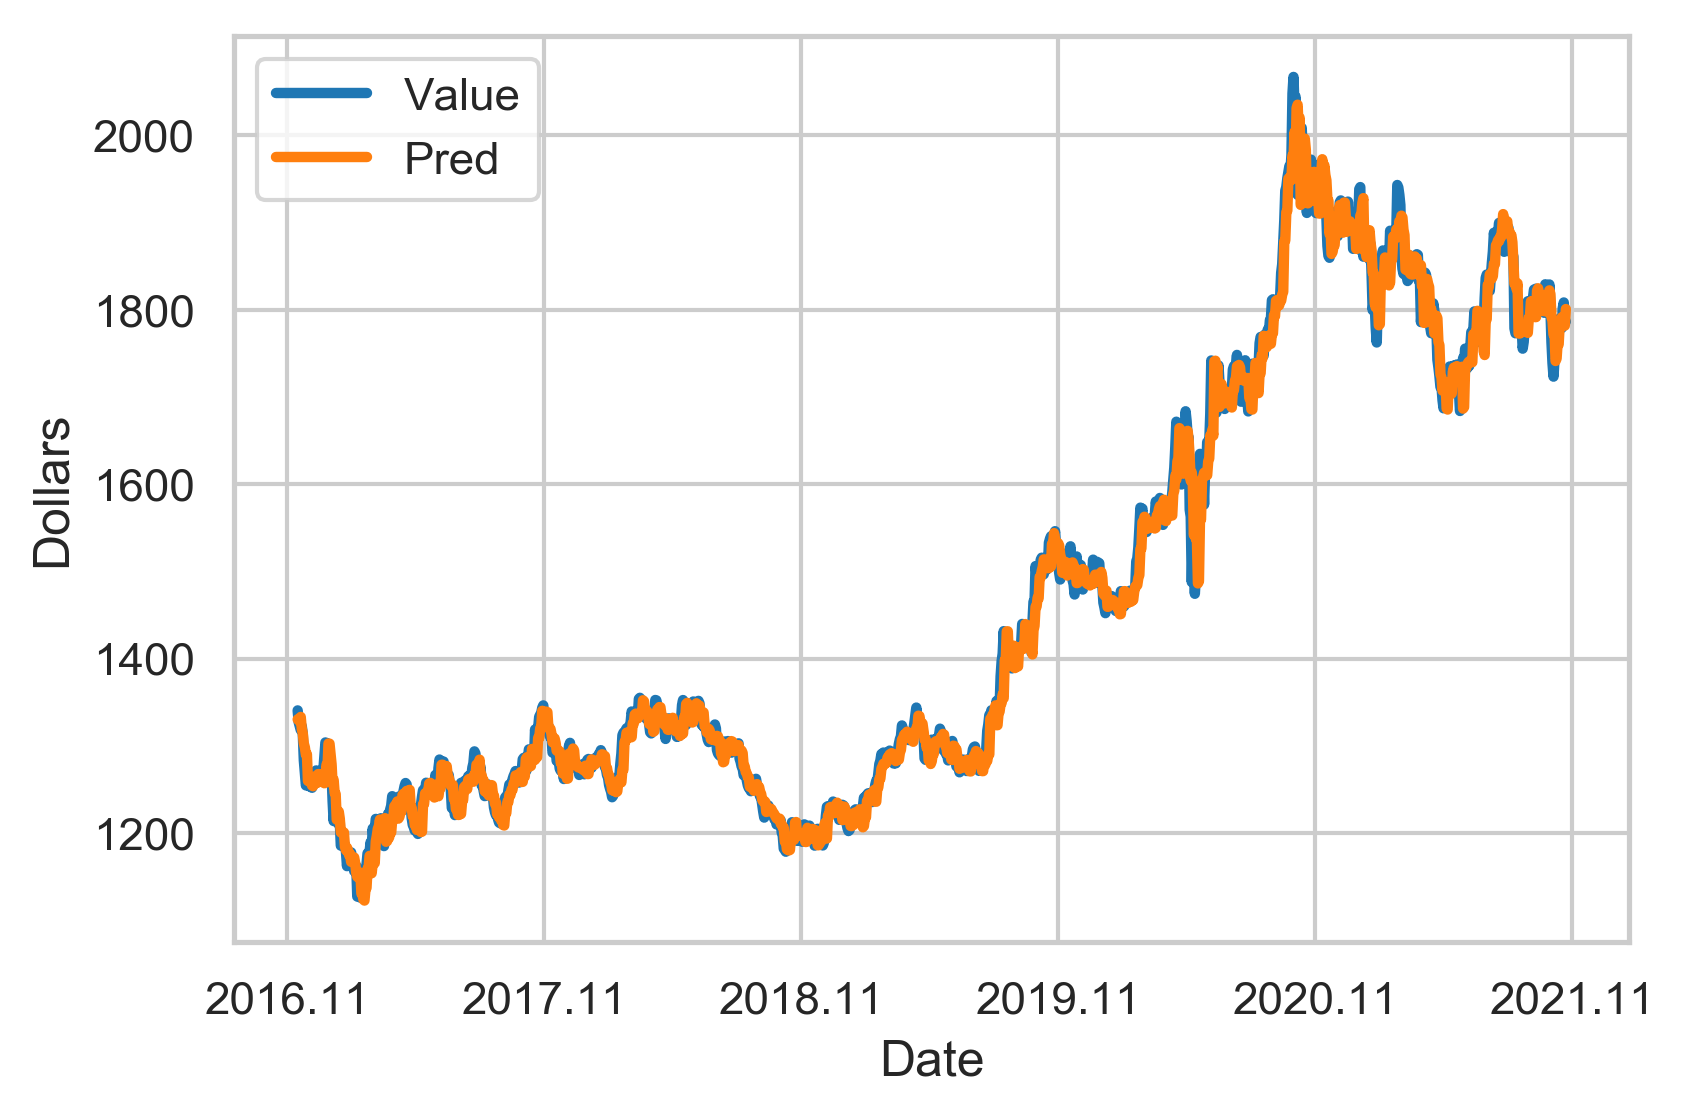
\includegraphics[scale=0.5]{lstm_gold}
		\end{minipage}
	}
	\subfigure[Bitcoin price forecasting by LSTM model]
	{
		\begin{minipage}{7cm}
			\centering
			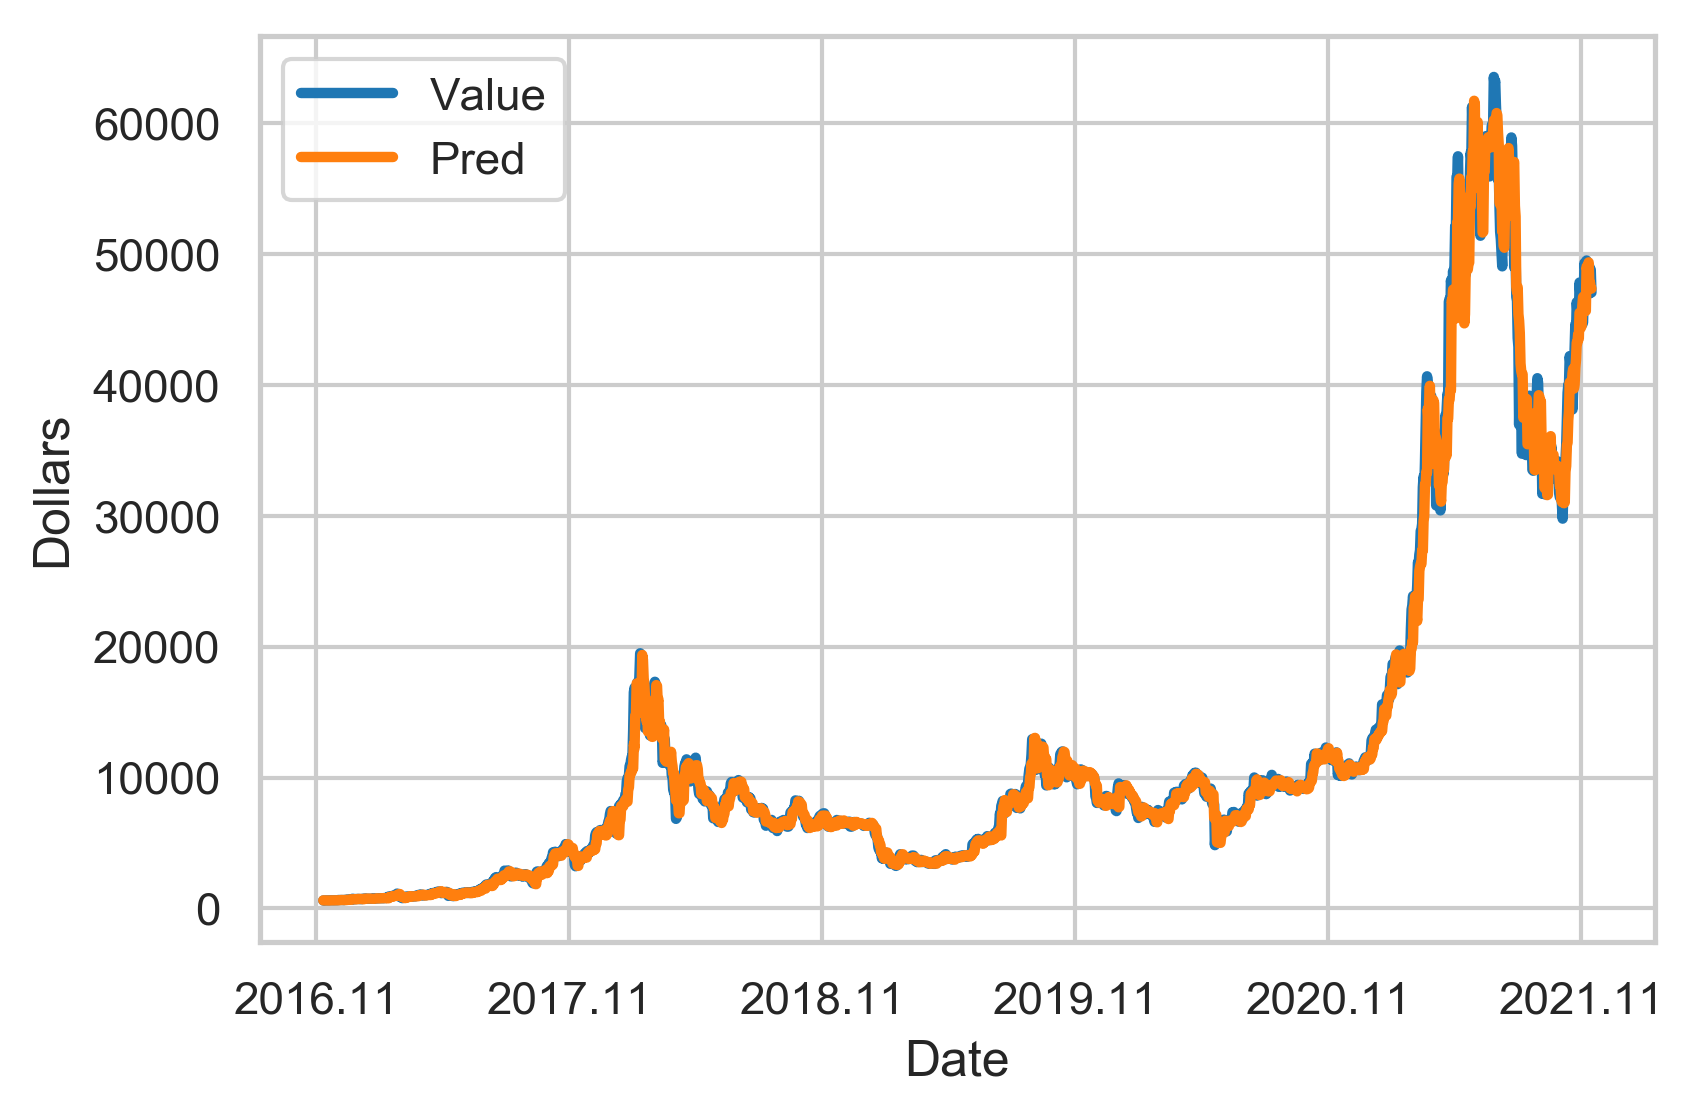
\includegraphics[scale=0.5]{lstm_bc}
		\end{minipage}
	}
	\caption{LSTM prediction results}
	\label{fig:predict_new}
\end{figure}

Our basic investing framework is to buy assets when the expected future price is greater than the commission rate and sell assets when the predicted future price is lower, ensuring a rising trend in total assets. We use E-Ratio to find the best moment to open a position. And then we design a proprietary metric investment factor to measure a portfolio's gold-bitcoin allocation, asset purchases, and risk management. Daily return can be guaranteed at a low risk by optimizing the portfolio according to this indicator.
After a 5-year investment period, we can achieve a 129.6\% average yearly return. The trends in total assets over the five-year period are shown below
\begin{figure}[H]	%浮动体参数
	\centering
	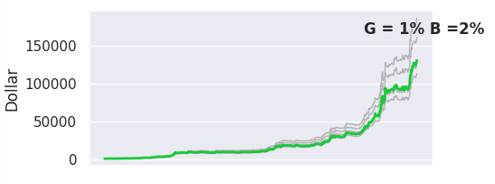
\includegraphics[width=0.5\textwidth]{nice}	%指定相同图片宽度,等比缩放
	\caption{Change in total assets (in USD)} 
	\label{fig:USD}		%题注、引用
\end{figure}
Additionally, our model outperforms other trading strategies. The radar chart below is constructed using the three indicators APR, Sharpe Ratio, and maximum drawdown.
\begin{figure}[H]	%浮动体参数
	\centering
	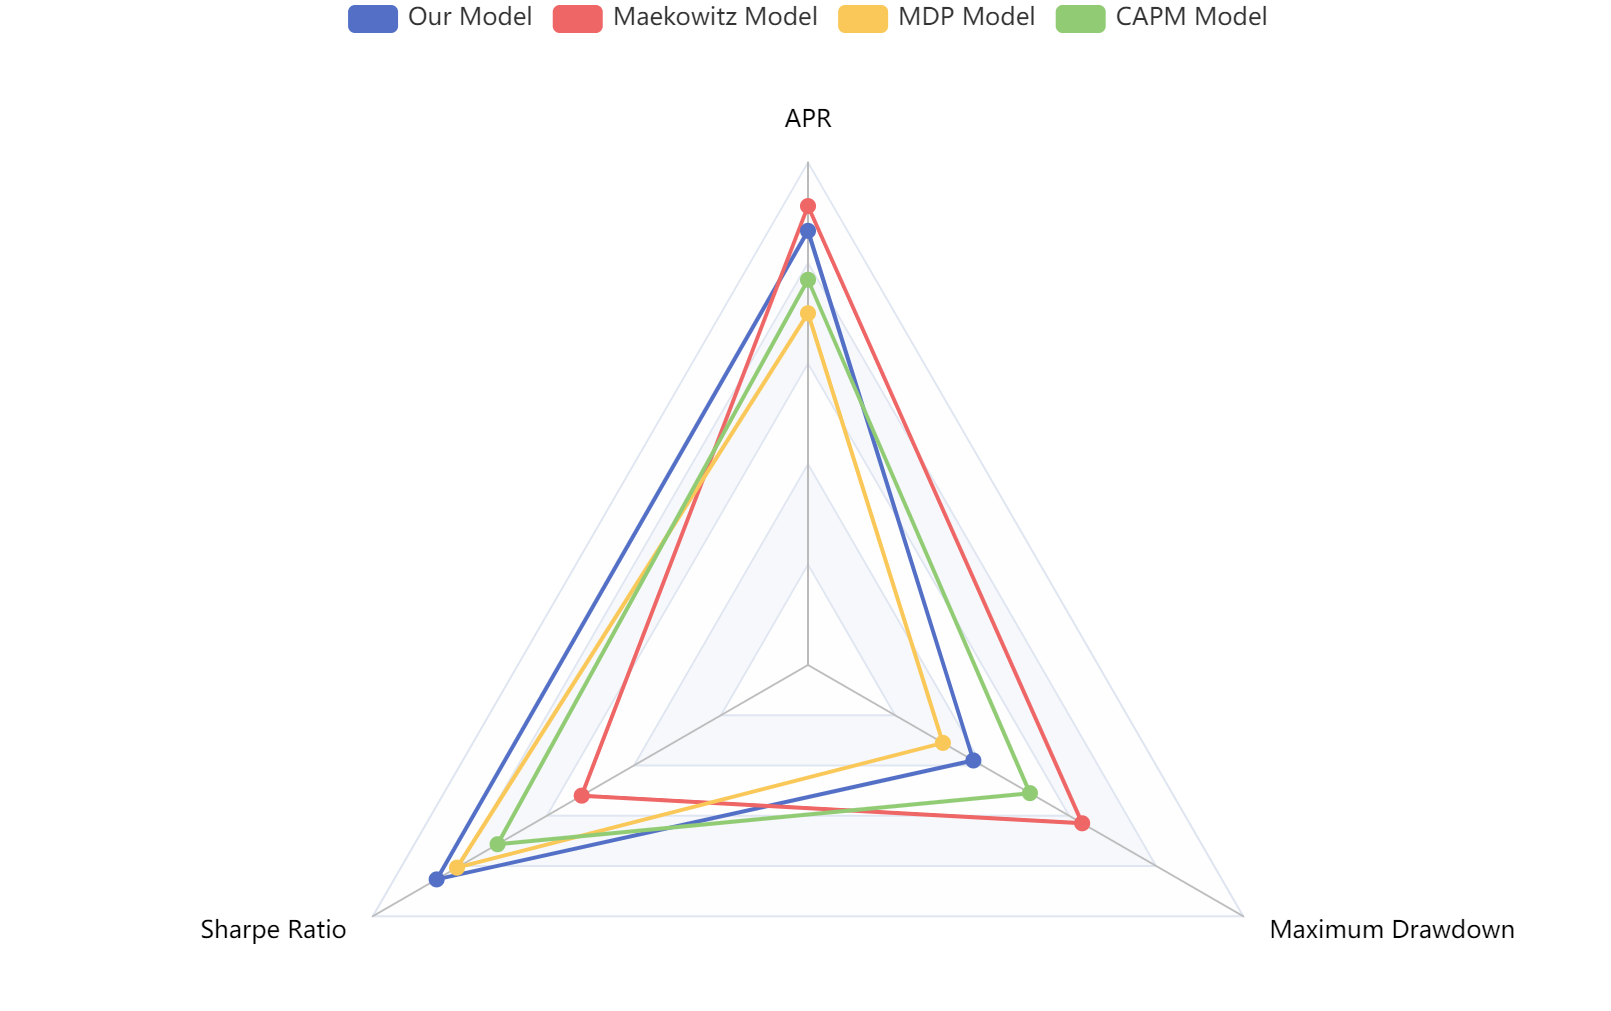
\includegraphics[height=0.4\textwidth]{radar}	%指定相同图片宽度,等比缩放
	\caption{Radar plot of model evaluation results} 
	\label{fig:radarnew}		%题注、引用
\end{figure}
From Fig.\ref{fig:radarnew}, we can know that our model has the highest APR and Sharpe ratio, and the maximum 30-day retracement is less than 40\%, proving that it offers the best return with the least risk among these strategies.

We have also evaluated the influence of commission changes on model returns and strategies, and our experiments show that commission changes have no impact on long-term returns. The total asset trend remains unchanged, but the allocation ratio of the two assets may be altered. Because of this, our models can reliably create earnings for you regardless of commission adjustments.

Finally, we genuinely hope that our models will be beneficial to you and generate sustained value for you.
	
	
\end{memo}

















\begin{appendices}






Here are some programmes we used in our model as follow.\\

\textbf{\textcolor[rgb]{0.98,0.00,0.00}{Input python source:}}
\lstinputlisting[language=Python]{./code/11.py}
\lstinputlisting[language=Python]{./code/1.py}

\end{appendices}


\bibliographystyle{unsrt}
\bibliography{book}
\end{document}
